\chapter{Performances of Different Numerical Methods}
\label{chapterPerformances}
As seen in chapter~\ref{chapter_caseStudy}, the only method used to study the model under consideration is the MPO method. However, other two methods have been analyzed and implemented for the same purpose, but with different performances: the QT method has been useful only for size chain of 8 and 10 sites, i.e. it has been useful in order to compare the MPO results and to confirm their plausibility, while CSR method has revealed not to be a suitable method for the study of this kind of models. In the present chapter, we show the limitations of CSR method for the case of 4-sites chain (for which we can perform a direct numerical integration of the master equation) and in the following section, a comparison between QT and MPO results is shown, with a brief analysis of their convergence and numerical errors.

\section{The CSR Method: Limitations and Usability}
The CSR method, described in section~\ref{chapter3_csr}, has been studied and implemented in order to analyze the model described in the last section. The algorithm is written in pseudocode in appendix~\ref{AppendixA}.

In this section, we show that the CSR method is not a fitting method for investigating systems described by a model such as the one under consideration.

In order to prove this, we can see the case of a 4-sites chain for the proposed model. In particular, we can study the magnetization profile along z direction, i.e. the steady-state expectation value $\langle \sigma_i^z \rangle$ of the Pauli spin- matrix $\sigma^z$ for each site:
\begin{equation*}
    \langle \sigma_i^z \rangle = \Tr(\sigma_i^z \rho_S),
\end{equation*}
being $\rho_S$ the steady-state density matrix of the system.

A chain made up by 4 spin-1/2 is characterized by a Hilbert space $\mathcal{H}$ with dimension $2^{4}$, so the number of states that describe the system are $2^4$. If the method works, the system will be described by a number of states $M < \dim(\mathcal{H})$, i.e. $M < 16$, in the case under consideration.

\begin{figure}[H]
    \centering
    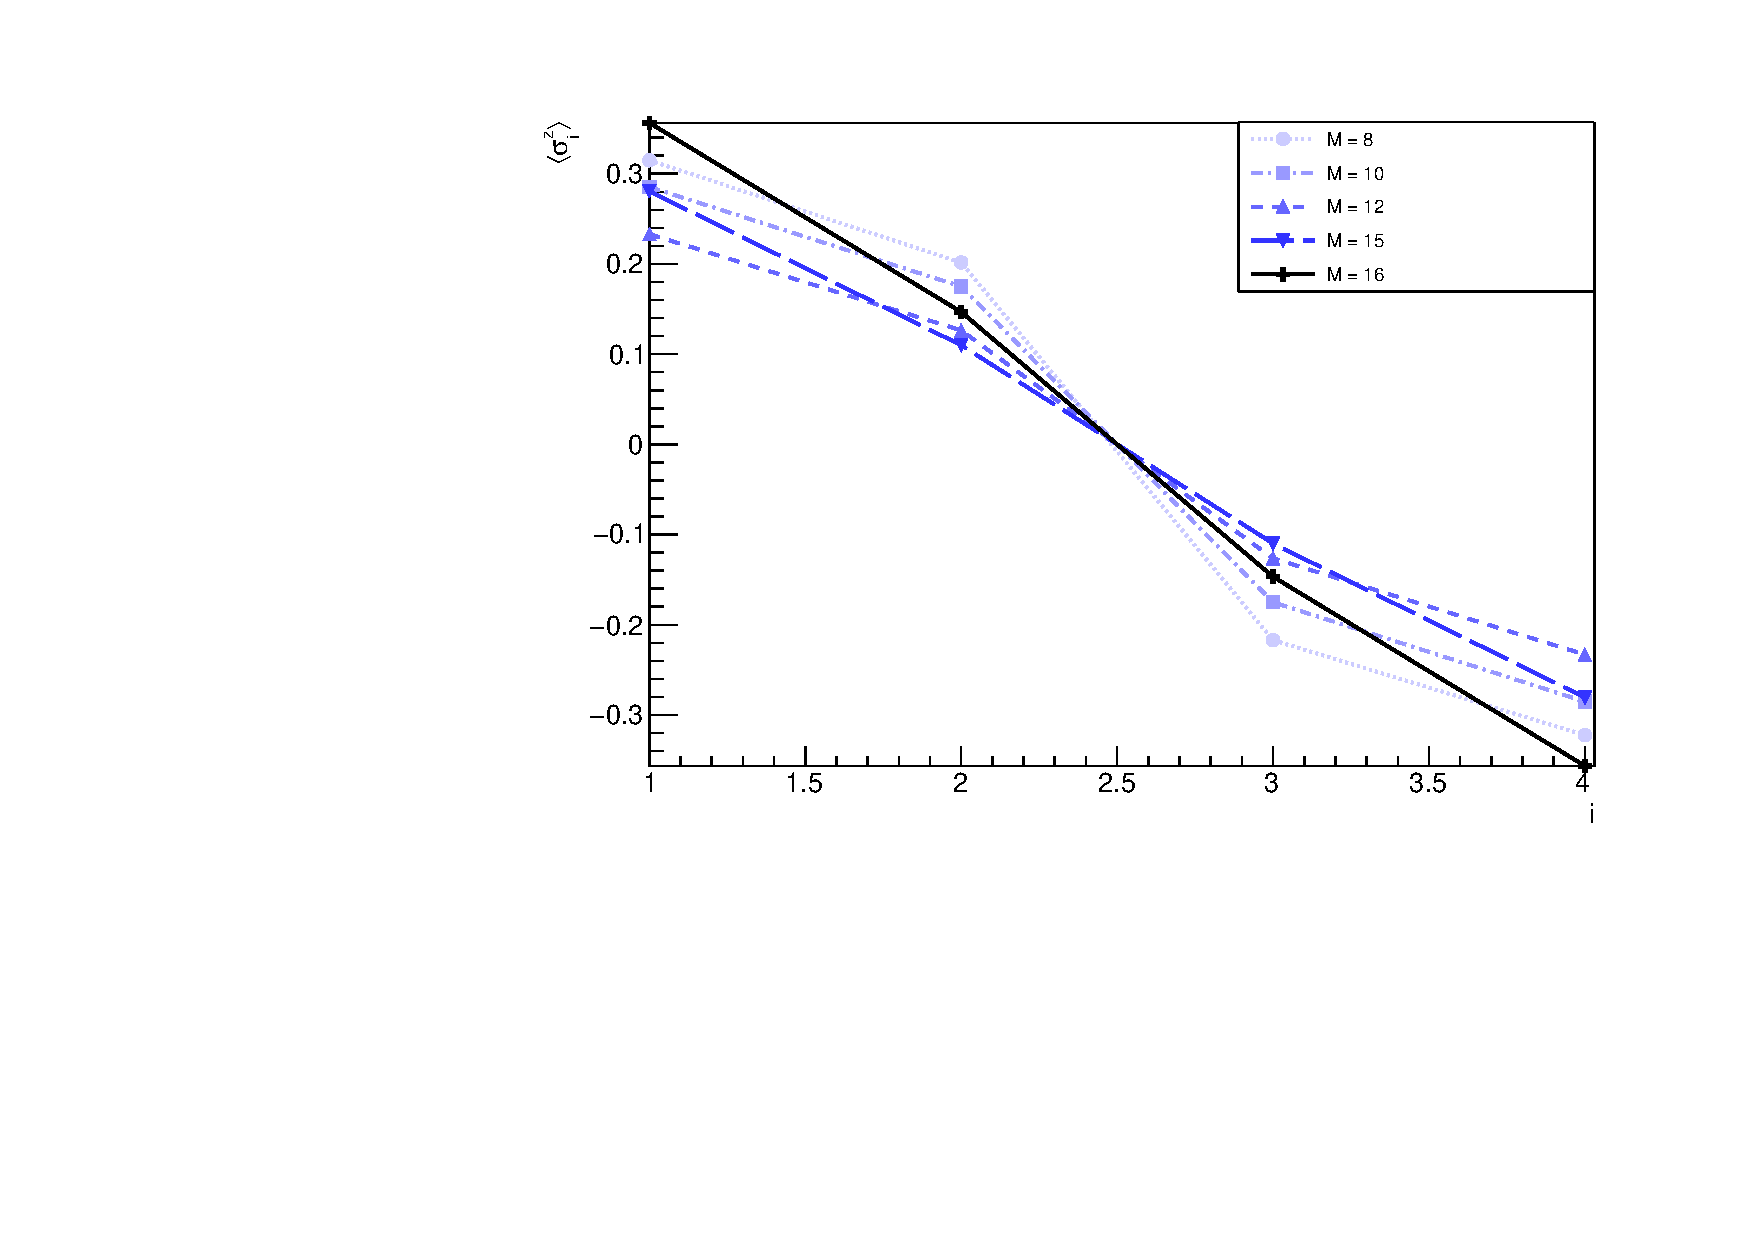
\includegraphics[scale=0.7]{Figures/4sites/4sites_LM_convergenceIncreasingM.pdf}
    \captionsetup{width=1.\linewidth}
    \caption{Spin profile of a 4-sites chain for the model described above with $J_z=1$ for several values of corner-space dimension $M$. The cyan markers are those representing the expectation value of the magnetization calculated by means of a complete set of states of Hilbert space (which has dimension $2^4$).}
    \label{fig:4sites_LM_convergenceIncreasingM}
\end{figure}

In figure~\ref{fig:4sites_LM_convergenceIncreasingM}, it is clear that for such a system the convergence has not been reached. Even for $M = 15$, that covers almost the total Hilbert space dimension, the results are not the convergent ones (shown in cyan).

On the other hand, if we consider a model in which every site is coupled to a dissipator, we can see how the magnetization profile gets to convergence starting from $M = 9$ already.


\begin{figure}[H]
    \centering
    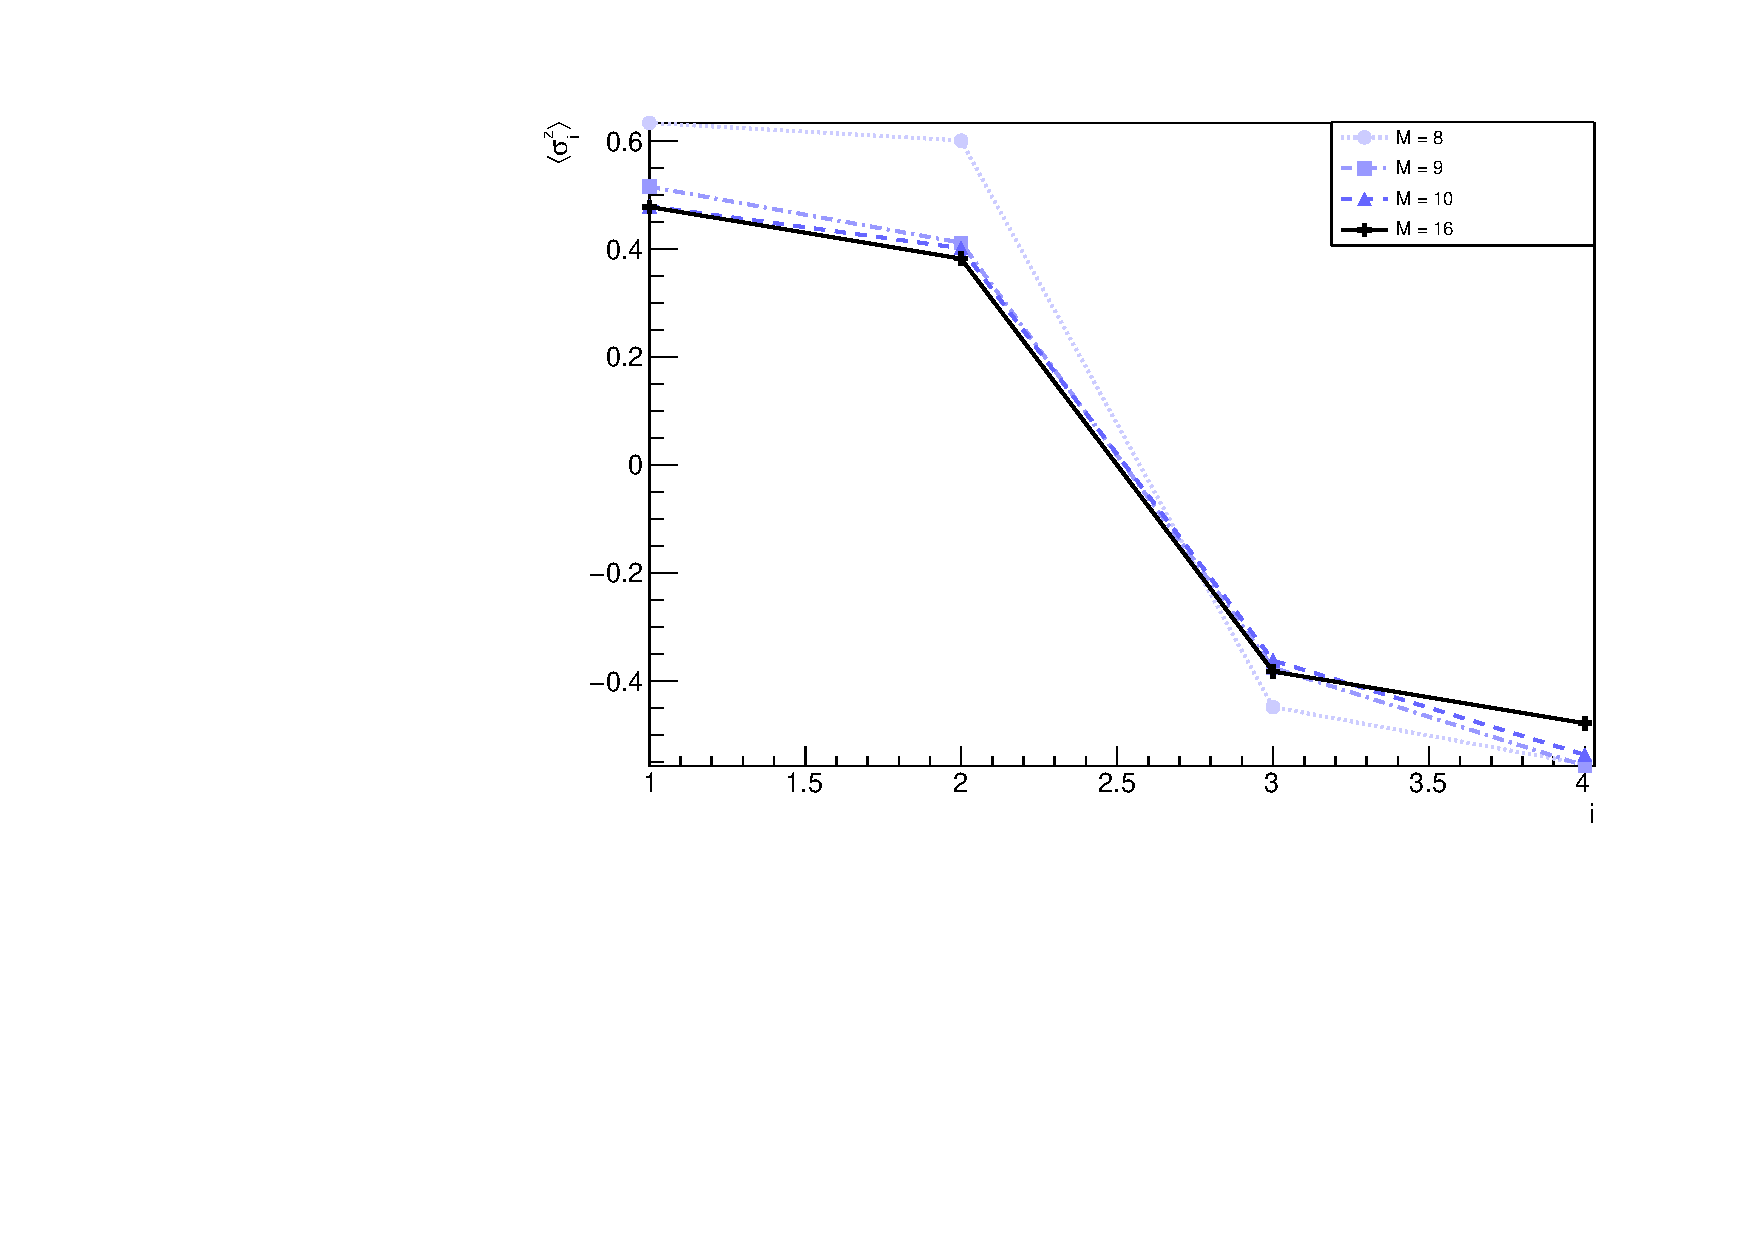
\includegraphics[scale=0.7]{Figures/4sites/4sites_totalDissipators.pdf}
    \captionsetup{width=1.\linewidth}
    \caption{Spin profile of a 4-sites chain in which every spin of the chain is coupled to a dissipator. In this case, the convergence is reached for $M<\text{dim}(\mathcal{H})$.}
    \label{fig:4sites_totalDissipators}
\end{figure}

In order to confirm the limitations of this method, the same comparison is done for a longer chain, made up by 8 sites. In this case, the results of CSR method are compared to those of MPO method, since a brute-force diagonalization of the Liouvillian operator would not be possible: it would require a huge amount of memory. We have reason to believe that the results obtained from MPO method are plausible, as we will see in the next sections.

\begin{figure}[H]
    \centering
    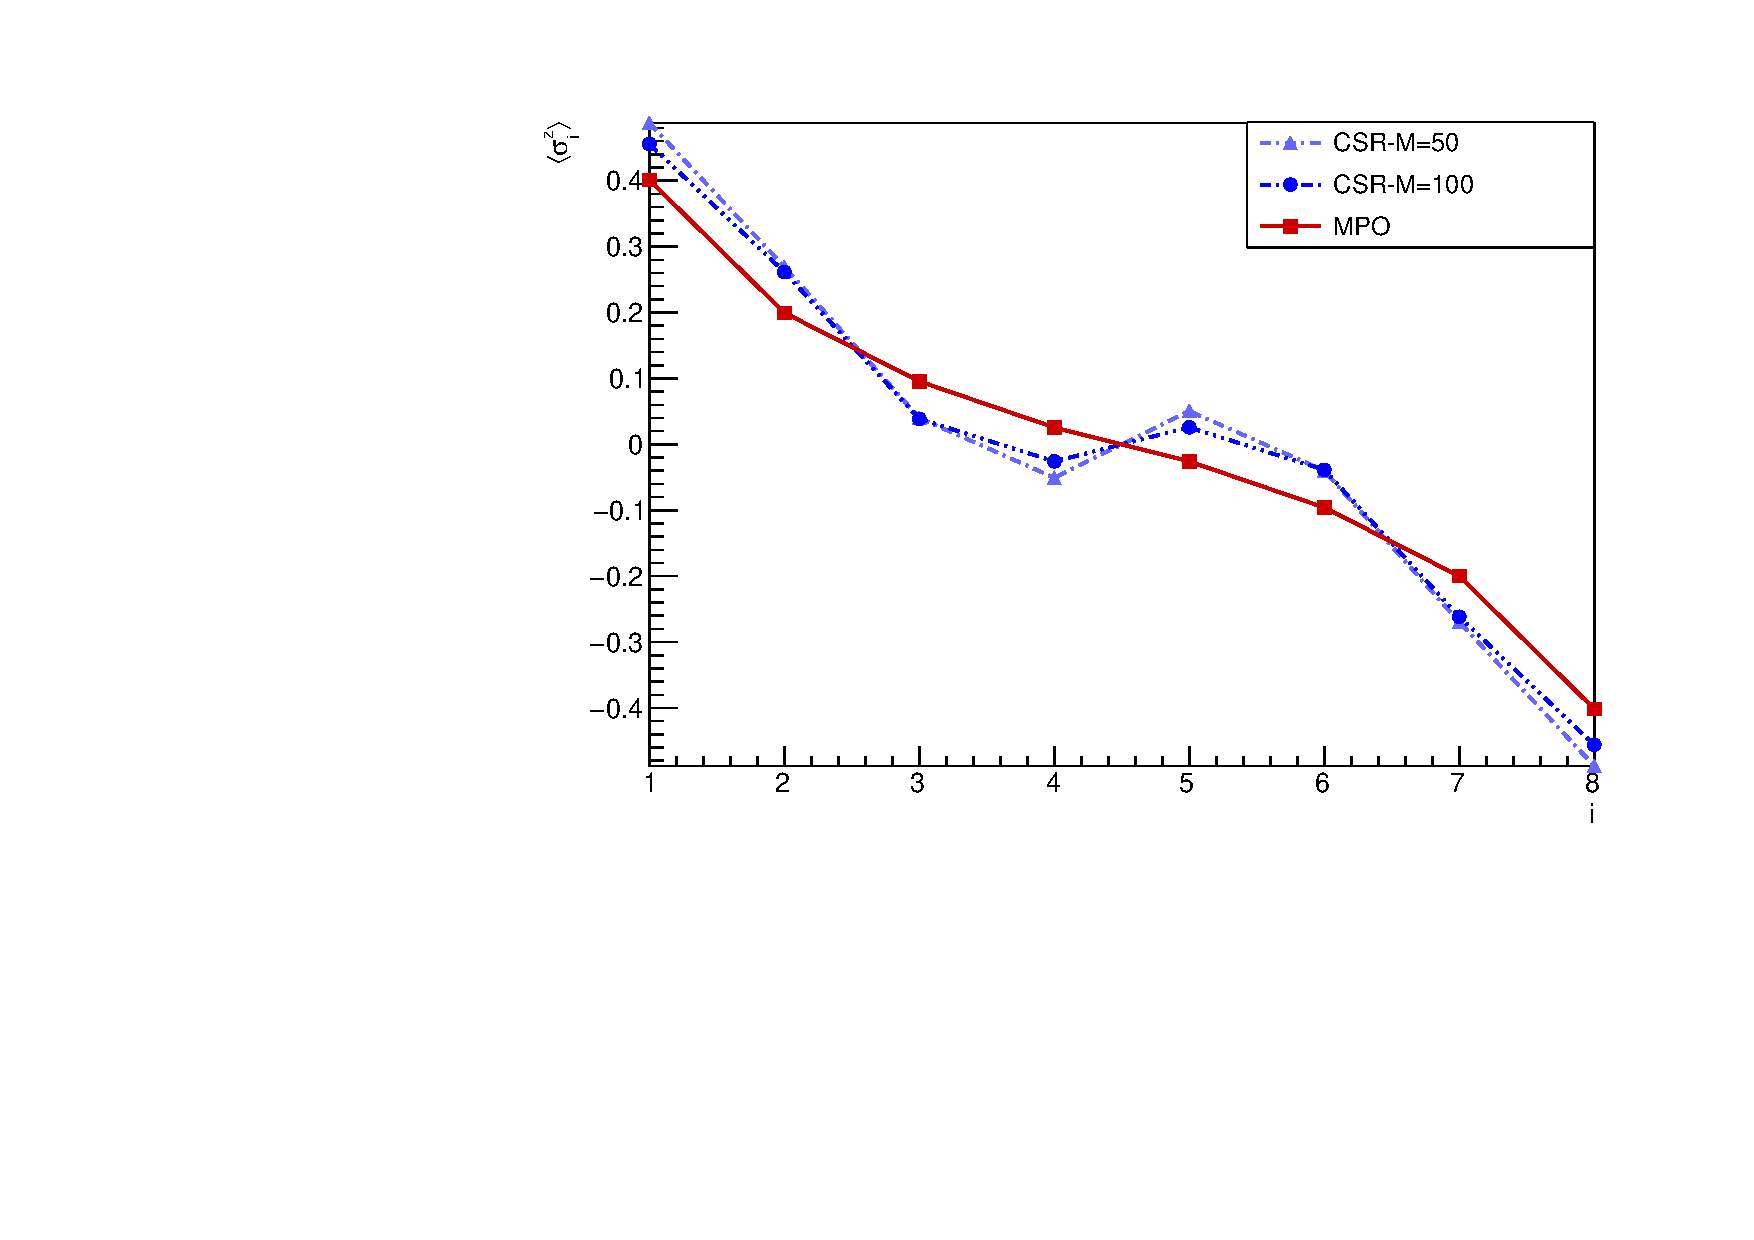
\includegraphics[scale=0.7]{Figures/8sites/1U1D_comparisonCSR_MPO_8site.pdf}
    \captionsetup{width=1.\linewidth}
    \caption{Spin profile of a 8-sites chain for the model described in sec.\ref{sec:model}. Significant differences between the data obtained for $M=50$ and $M=100$ are not noticed.}
    \label{fig:1U1D_comparisonCSR_MPO_8site}
\end{figure}

\begin{figure}[H]
    \centering
    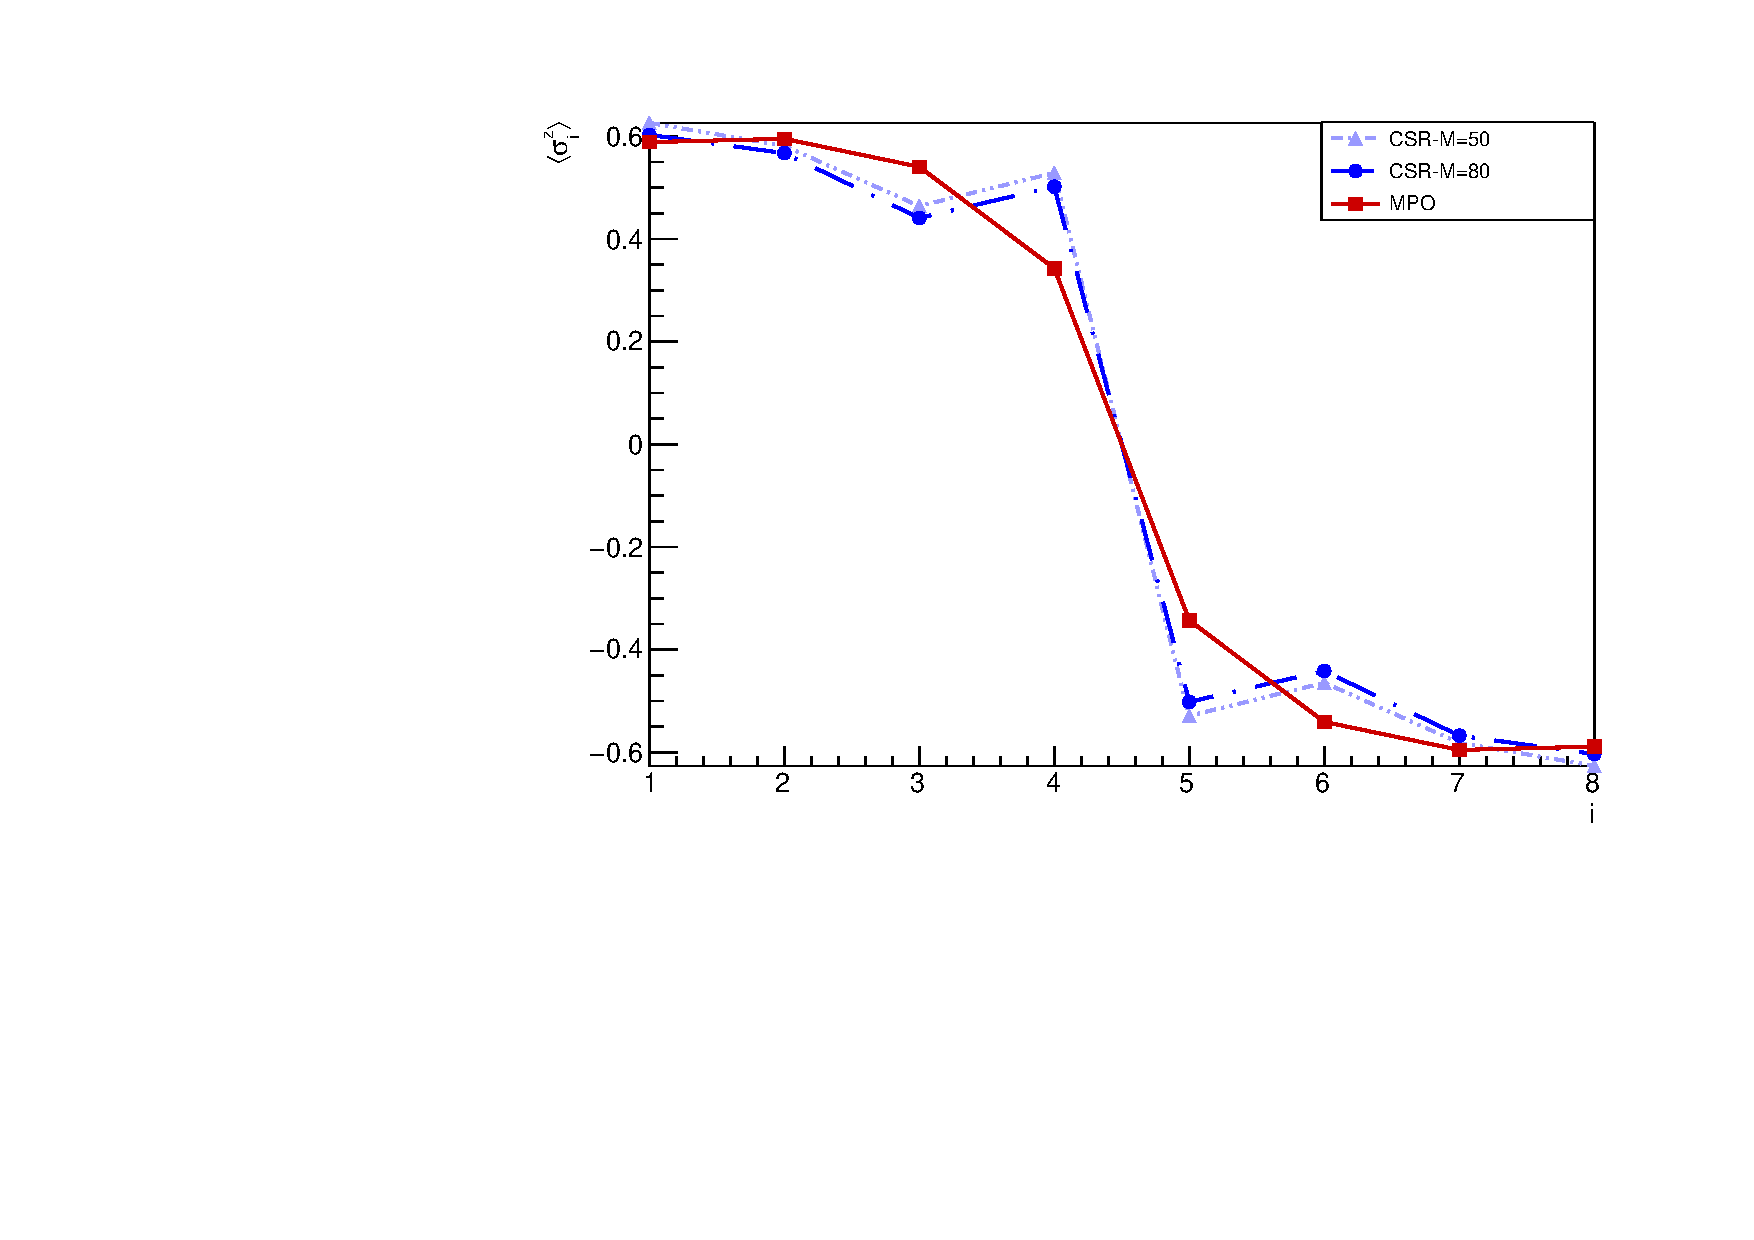
\includegraphics[scale=0.7]{Figures/8sites/8sites_MPOvsCORNER_4U4D.pdf}
    \captionsetup{width=1.\linewidth}
    \caption{Spin profile of a 8-sites chain in which every spin of the chain is coupled to a dissipator.}
    \label{fig:8sites_MPOvsCORNER_4U4D}
\end{figure}

In conclusion, in fig.~\ref{fig:LMComparison16s1051} it is displayed the magnetization profile of a 16-sites chain obtained by CSR and MPO methods.

\begin{figure}[H]
    \centering
    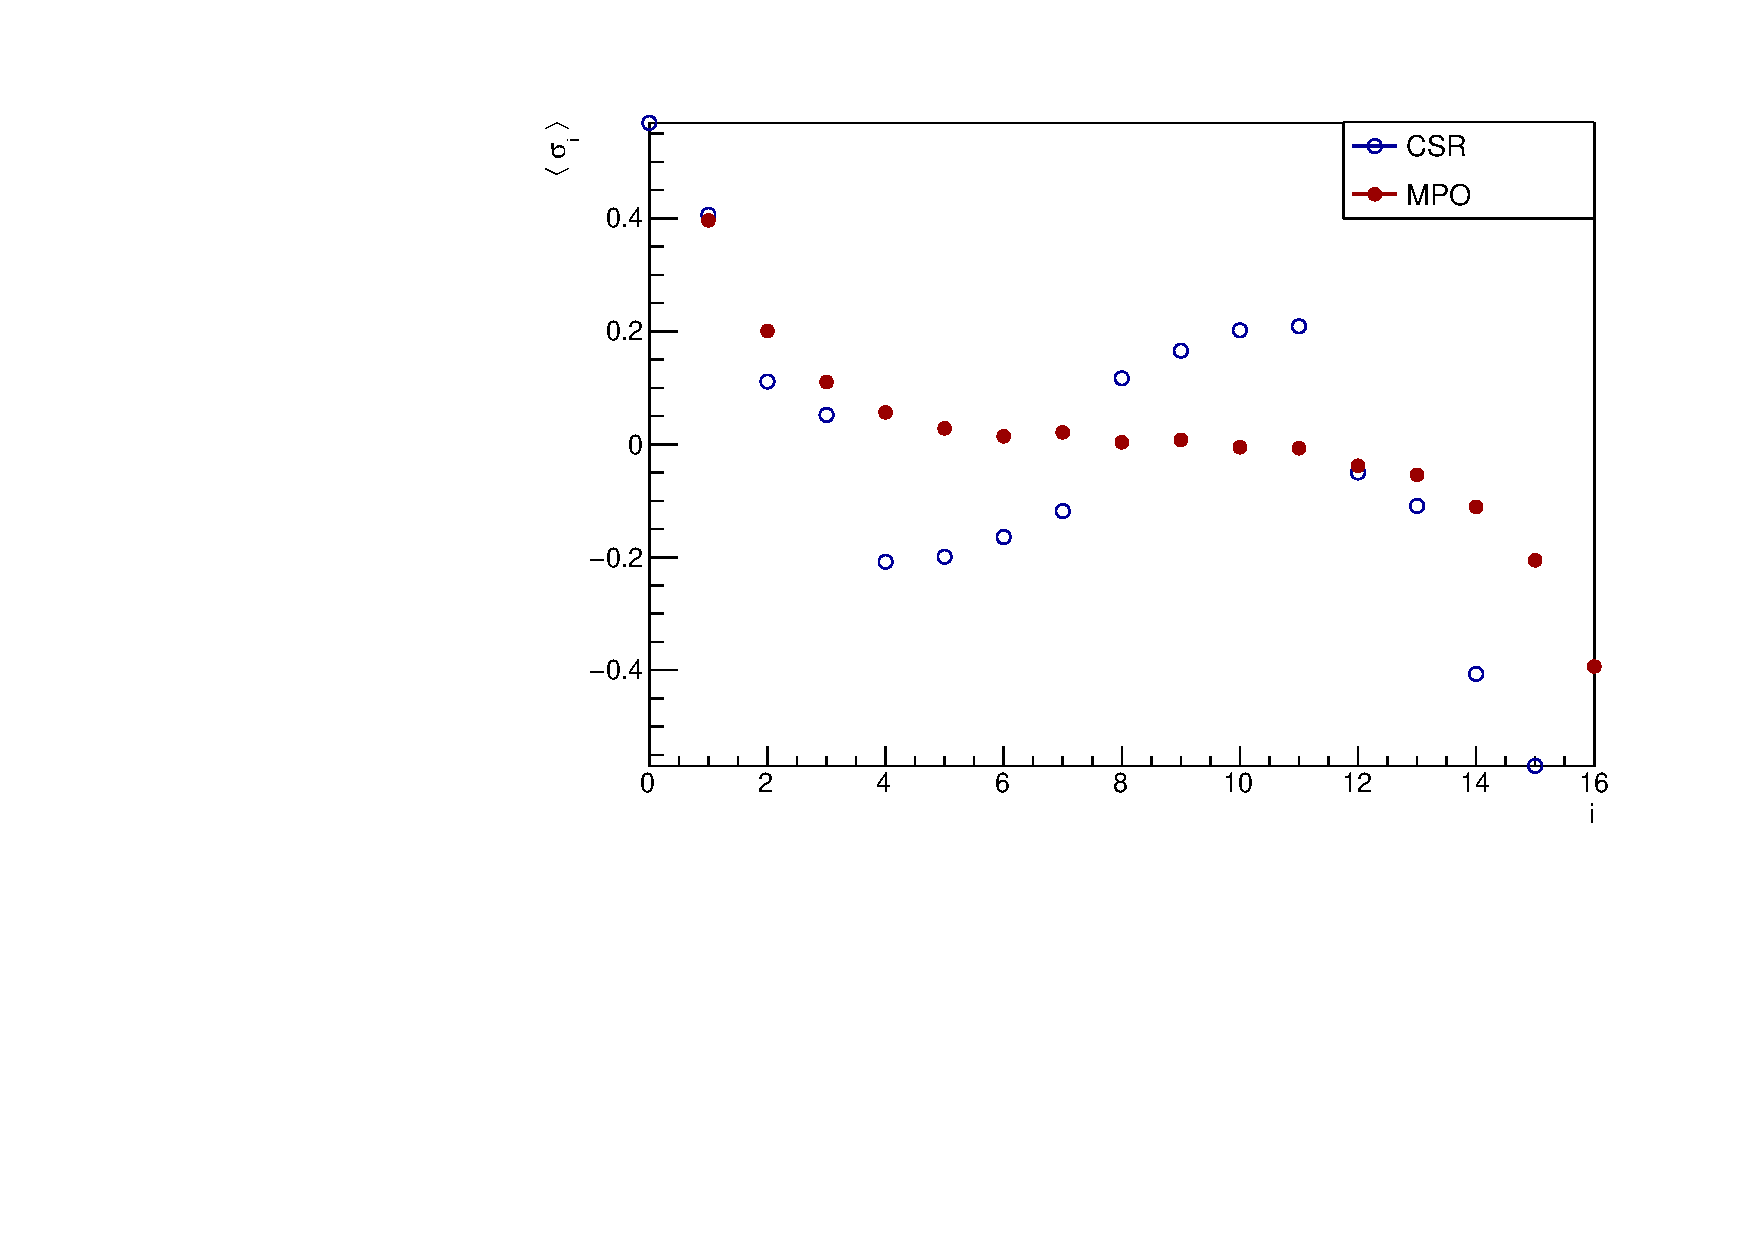
\includegraphics[scale=0.7]{Figures/16sites/LMComparison16s1051.pdf}
    \captionsetup{width=1.\linewidth}
    \caption{Spin profile for a 16-sites chain for the model described in section~\ref{sec:model}. Data in red are obtained from MPO method, with m = 80 and T = 2000 and data in blue are obtained from CSR method, with M = 65. It is self-evident the inadequacy of the corner-space method, for the model under study.}
    \label{fig:LMComparison16s1051}
\end{figure}

\begin{figure}[H]
    \centering
    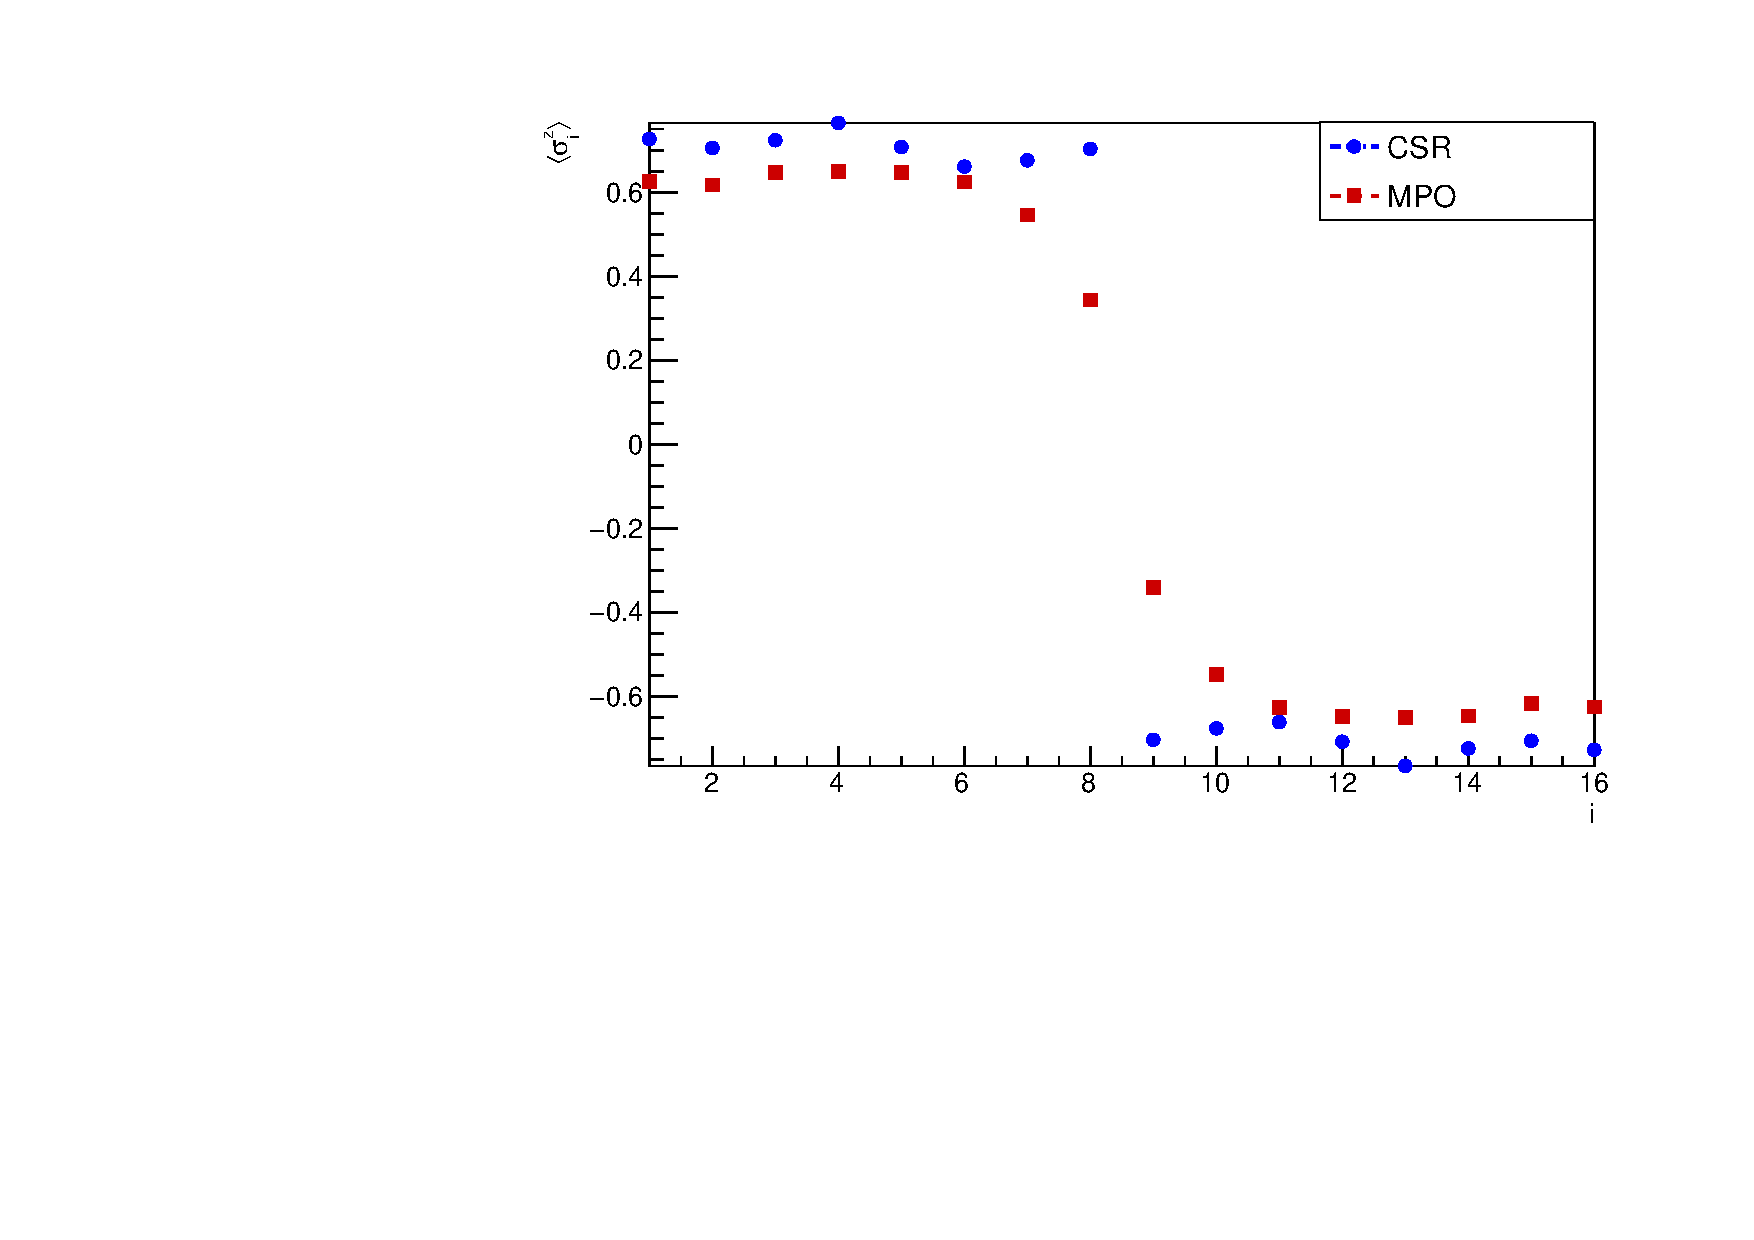
\includegraphics[scale=0.7]{Figures/8U8D_comparisonCSRvsMPO.pdf}
    \captionsetup{width=1.\linewidth}
    \caption{Spin profile for a 16-sites chain in which every spin of the chain is coupled to a dissipator. The dimension of the corner-space is $M=65$.}
    \label{fig:LMComparison16s1051}
\end{figure}

\section{The QT Method: Convergence and Numerical Errors}

In this section a brief discussion on the convergence of the data and error calculus is done. 

The QT method, explained in section~\ref{chapt3_qtm}, doing the stochastic unraveling of the master equation, builds the quantum trajectories after which it is named.  Every quantum trajectory corresponds to a simulated experiment and for the model under consideration, it has an oscillatory profile as that displayed in fig.~\ref{fig:SS_s8J10511}. In order to stabilize the solution, for every quantum trajectory, the average in time is considered, starting from the end of the transient, needed for a solution of the Lindblad equation to converge towards the steady-state.

\begin{figure}[H]
    \centering
    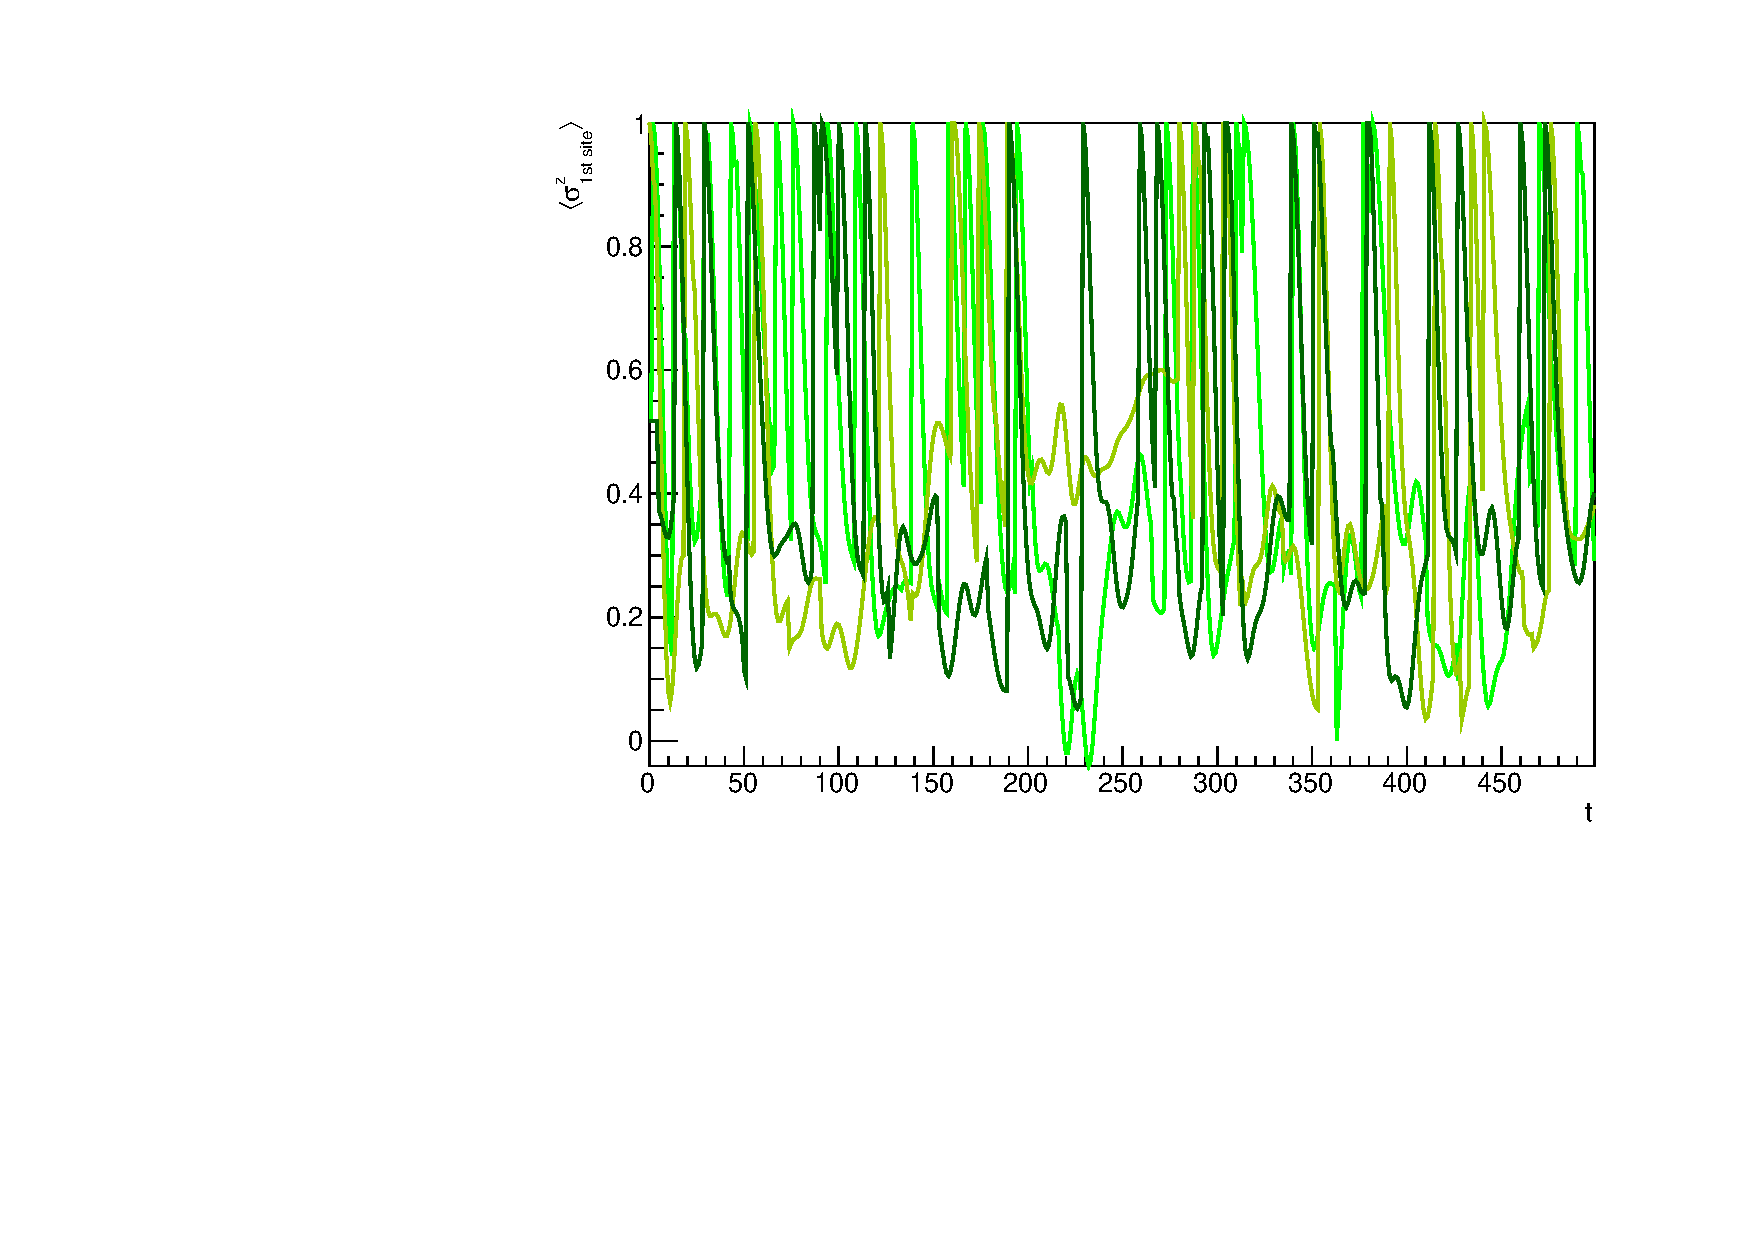
\includegraphics[scale=0.7]{Figures/QTrajectories3.pdf}
    \captionsetup{width=1.\linewidth}
    \caption{Example of three quantum trajectories; in particular, this is the expectation value of the magnetization of the first site of the chain, for $J_z = 1$ and $\gamma = 1$. The total elapsed time is $T=500$, while the time step $dt = 0.1$.}
    \label{fig:QTrajectories3}
\end{figure}

For the same case considered in fig.~\ref{fig:QTrajectories3}, the convergence of the mean values is shown in fig.~\ref{fig:Convergence_s8J1051}. 

\begin{figure}[H]
    \centering
    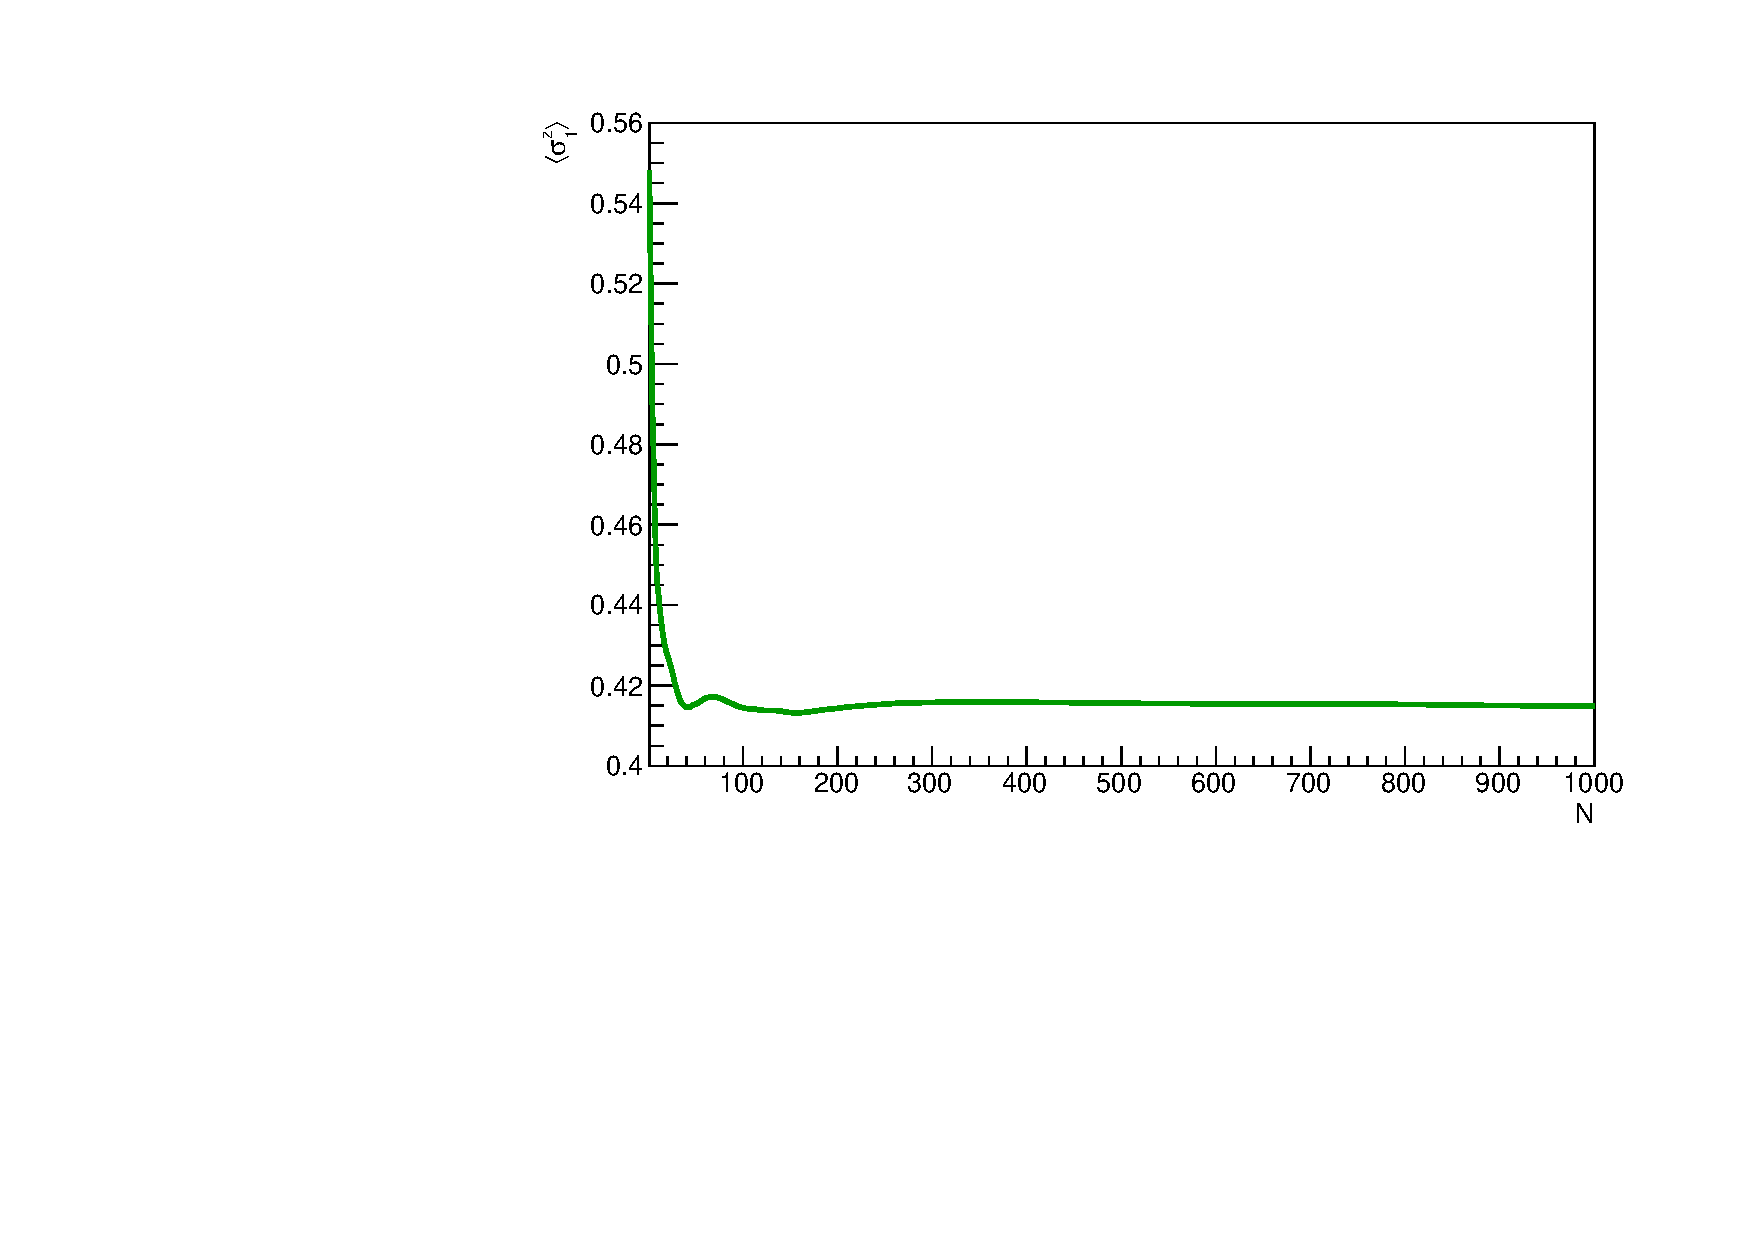
\includegraphics[scale=0.7]{Figures/Convergence_s8J1051.pdf}
    \captionsetup{width=1.\linewidth}
    \caption{Study of the convergence of the mean values of the quantum trajectories. For the case under consideration, the number of events is $N = 1000$.}
    \label{fig:Convergence_s8J1051}
\end{figure}

The study of the 8-sites chain was done with an elapsed time for every event of $T = 500$ and time-step $dt = 0.1$. The number of the simulated events is $N = 1000$.

As an error it has been consider the standard deviation of the mean, i.e.
\begin{equation*}
    \sigma_{\text{mean}} = \frac{\sigma}{\sqrt{N}},
\end{equation*}
where $\sigma$ is the standard deviation of the mean in time in the quantum trajectory.

\section{The MPO Method: Convergence and Numerical Errors}
The convergence of MPO method depends essentially on the setting of two parameters: the bond dimension and the number of Trotter steps. The fig.~\ref{fig:convergenceMPO_8sites} shows the convergence profile for a 8-sites chain for $J_z = 1$ and $\gamma = 1$. The same quantity can reach convergence in different times if, for example, $J_z$ assumes another value. 

In the present work, for 8-sites chain it was considered a bond dimension $m = 100$ and Trotter steps in the range $[1200, 1500]$; for 12-sites chain it was considered a bond dimension $m = 60$ and Trotter steps in the range $[1000, 2000]$; for 16-sites chain it was considered a bond dimension $m = 80, 100$ and Trotter steps in the range $[1000, 1500]$.

In fig.~\ref{fig:convergence_8_12_16} the convergence of $\sigma^z$ for the first site of 8, 12, 16-sites chains. 

\begin{figure}[H]
\centering
\begin{subfigure}{\columnwidth}
\centering
    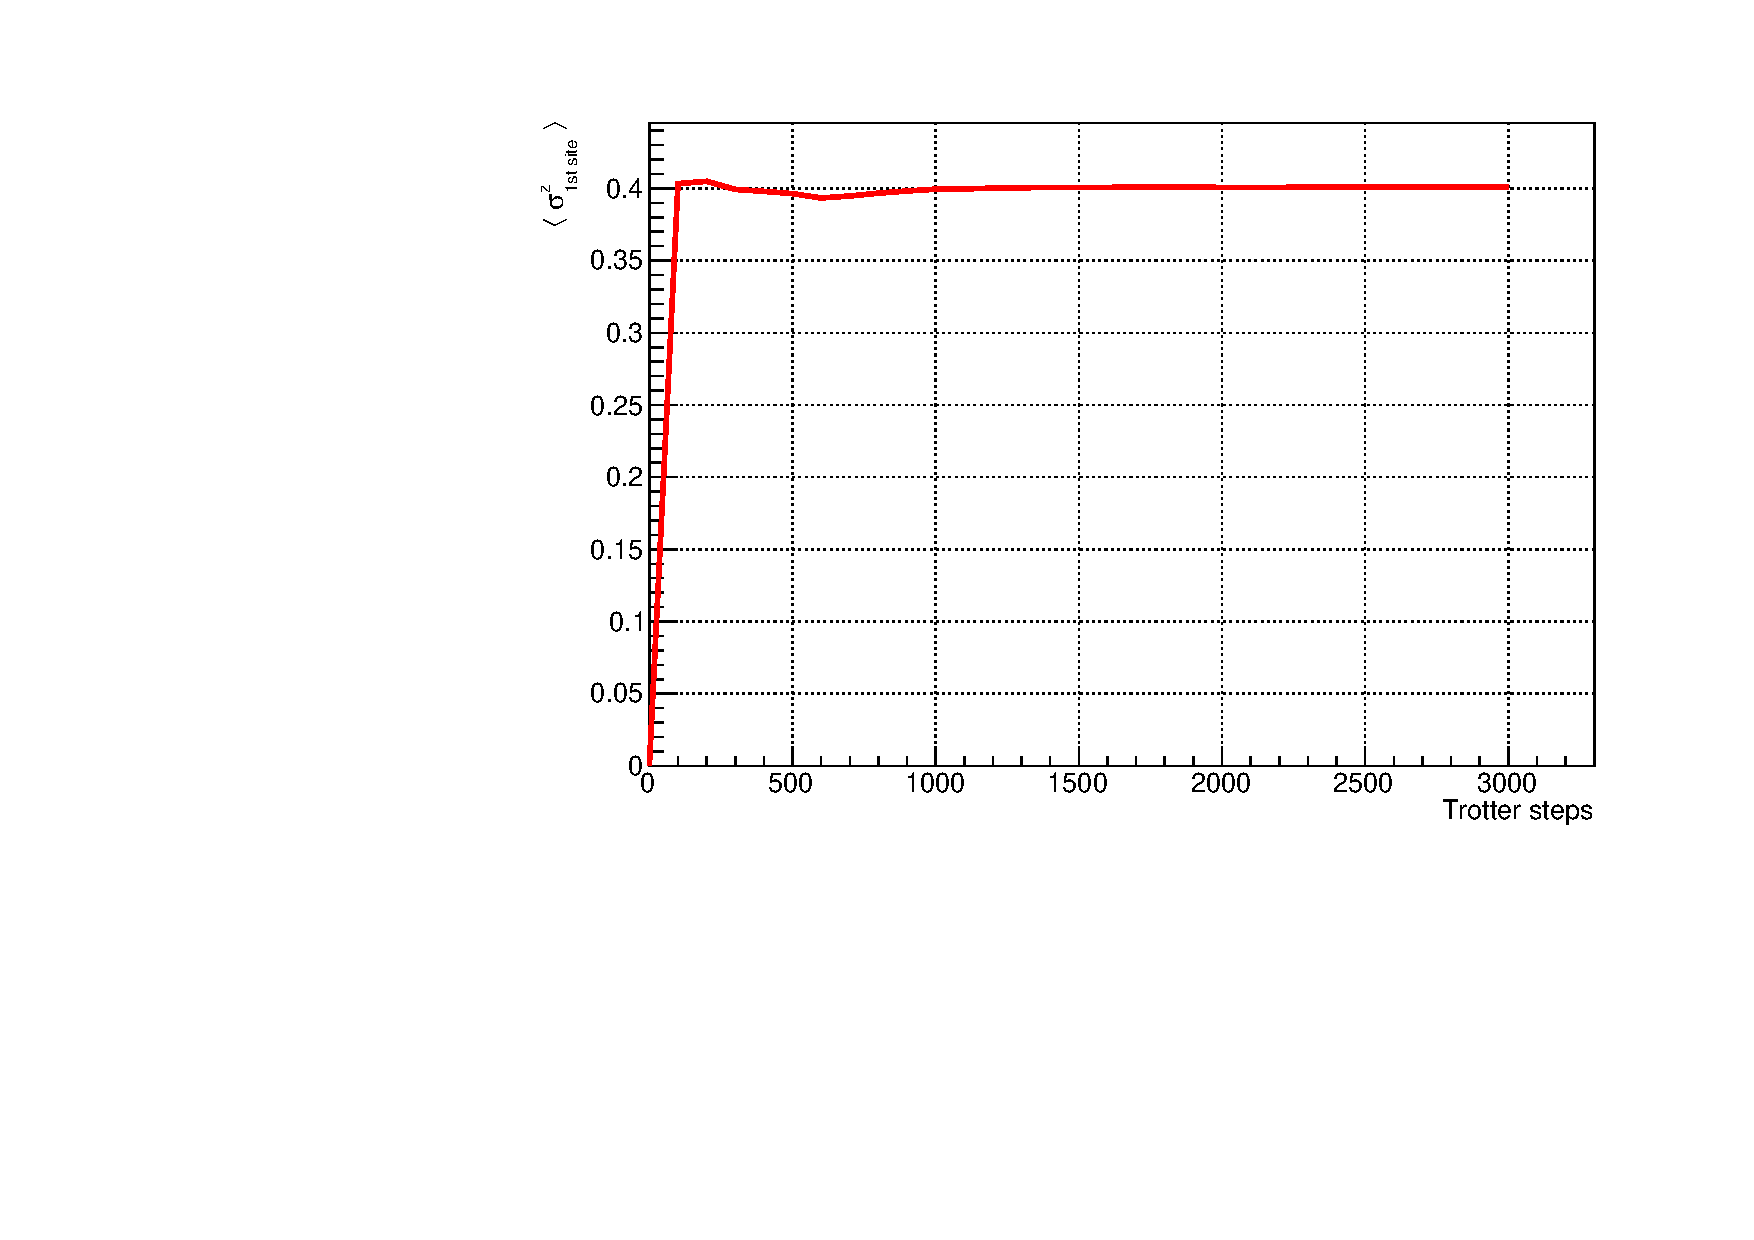
\includegraphics[scale=0.6]{Figures/convergence/Convergence_s8T3000J1051.pdf}
    \label{fig:8sites_LMvsGamma}
\end{subfigure}\quad
\begin{subfigure}{\columnwidth}
\centering
    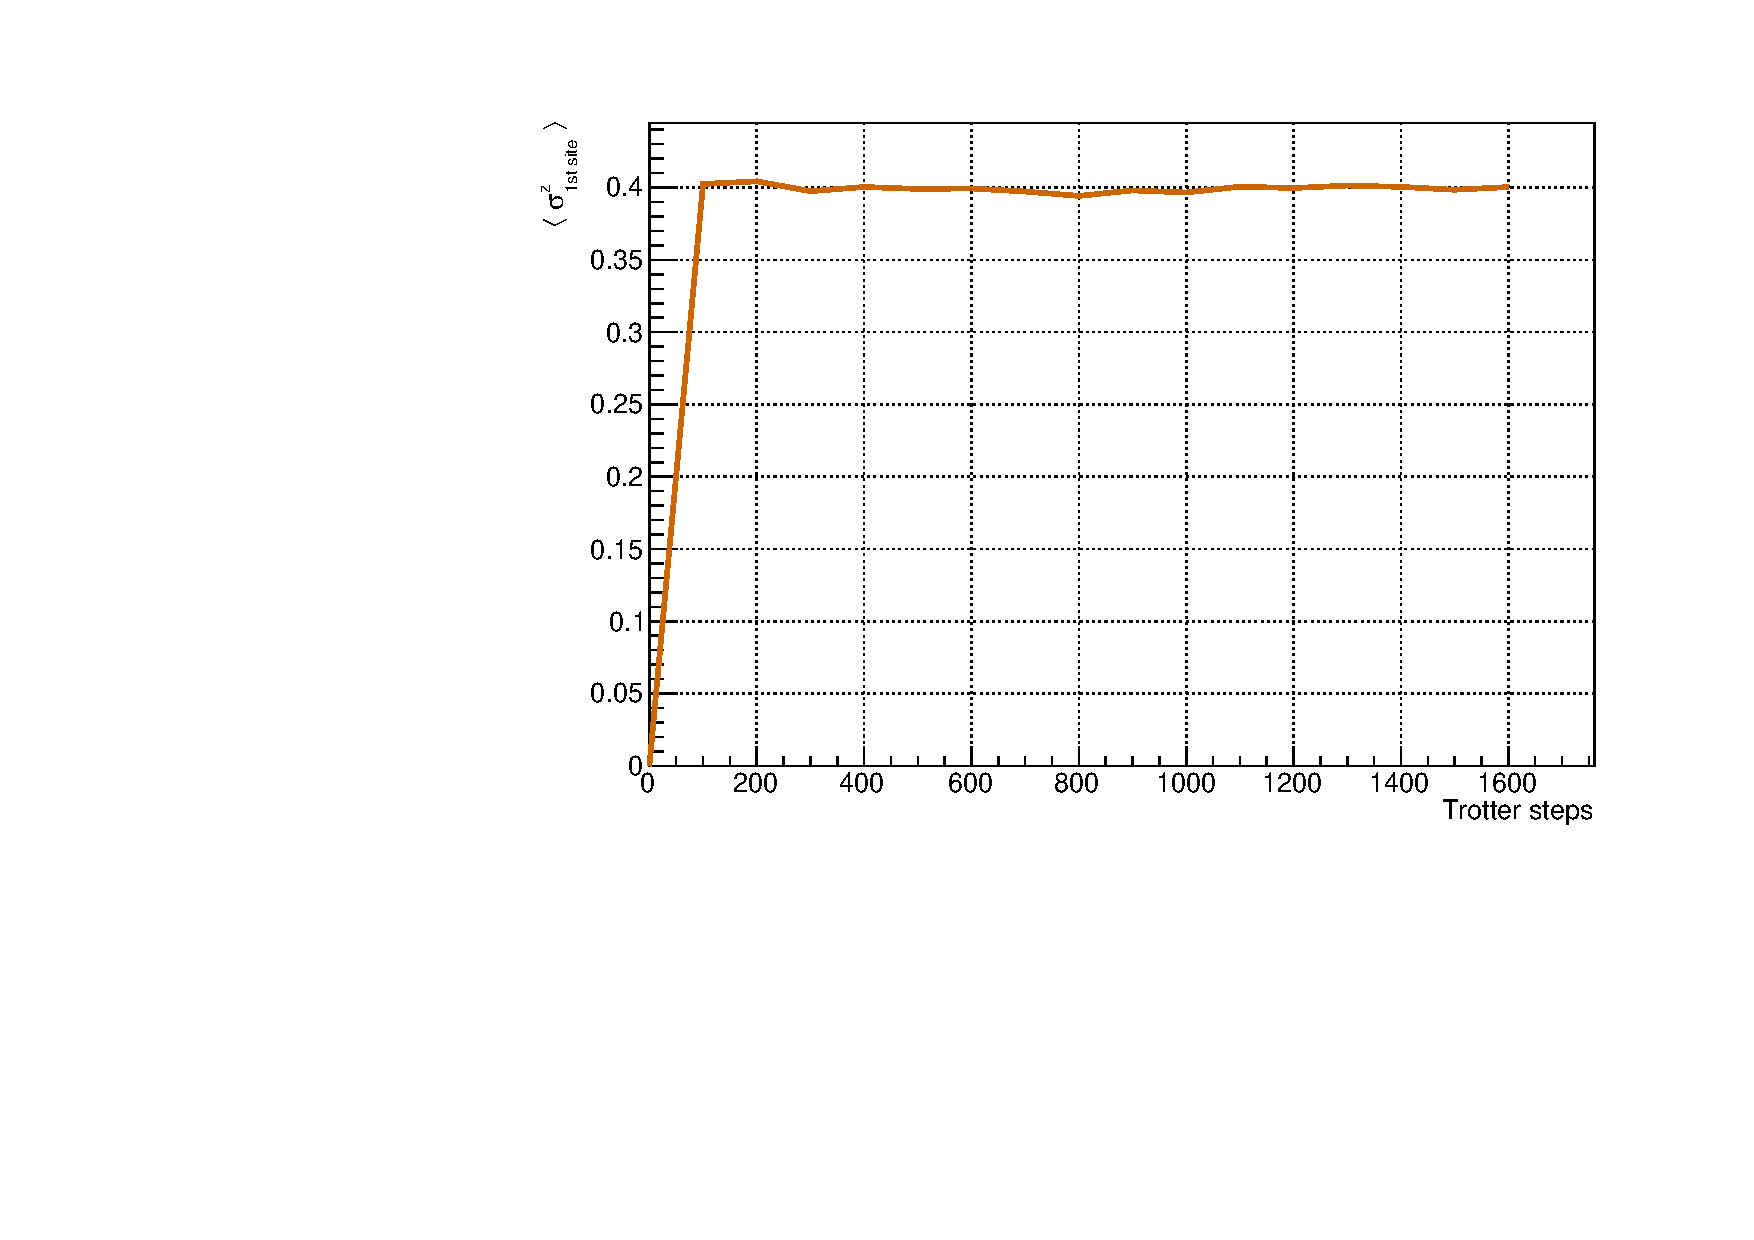
\includegraphics[scale=0.6]{Figures/convergence/Convergence_LM_L012_m060_Time001600_J1051.pdf}
    \label{fig:12sites_LMvsGamma}
\end{subfigure}\\
\begin{subfigure}{\columnwidth}
\centering
    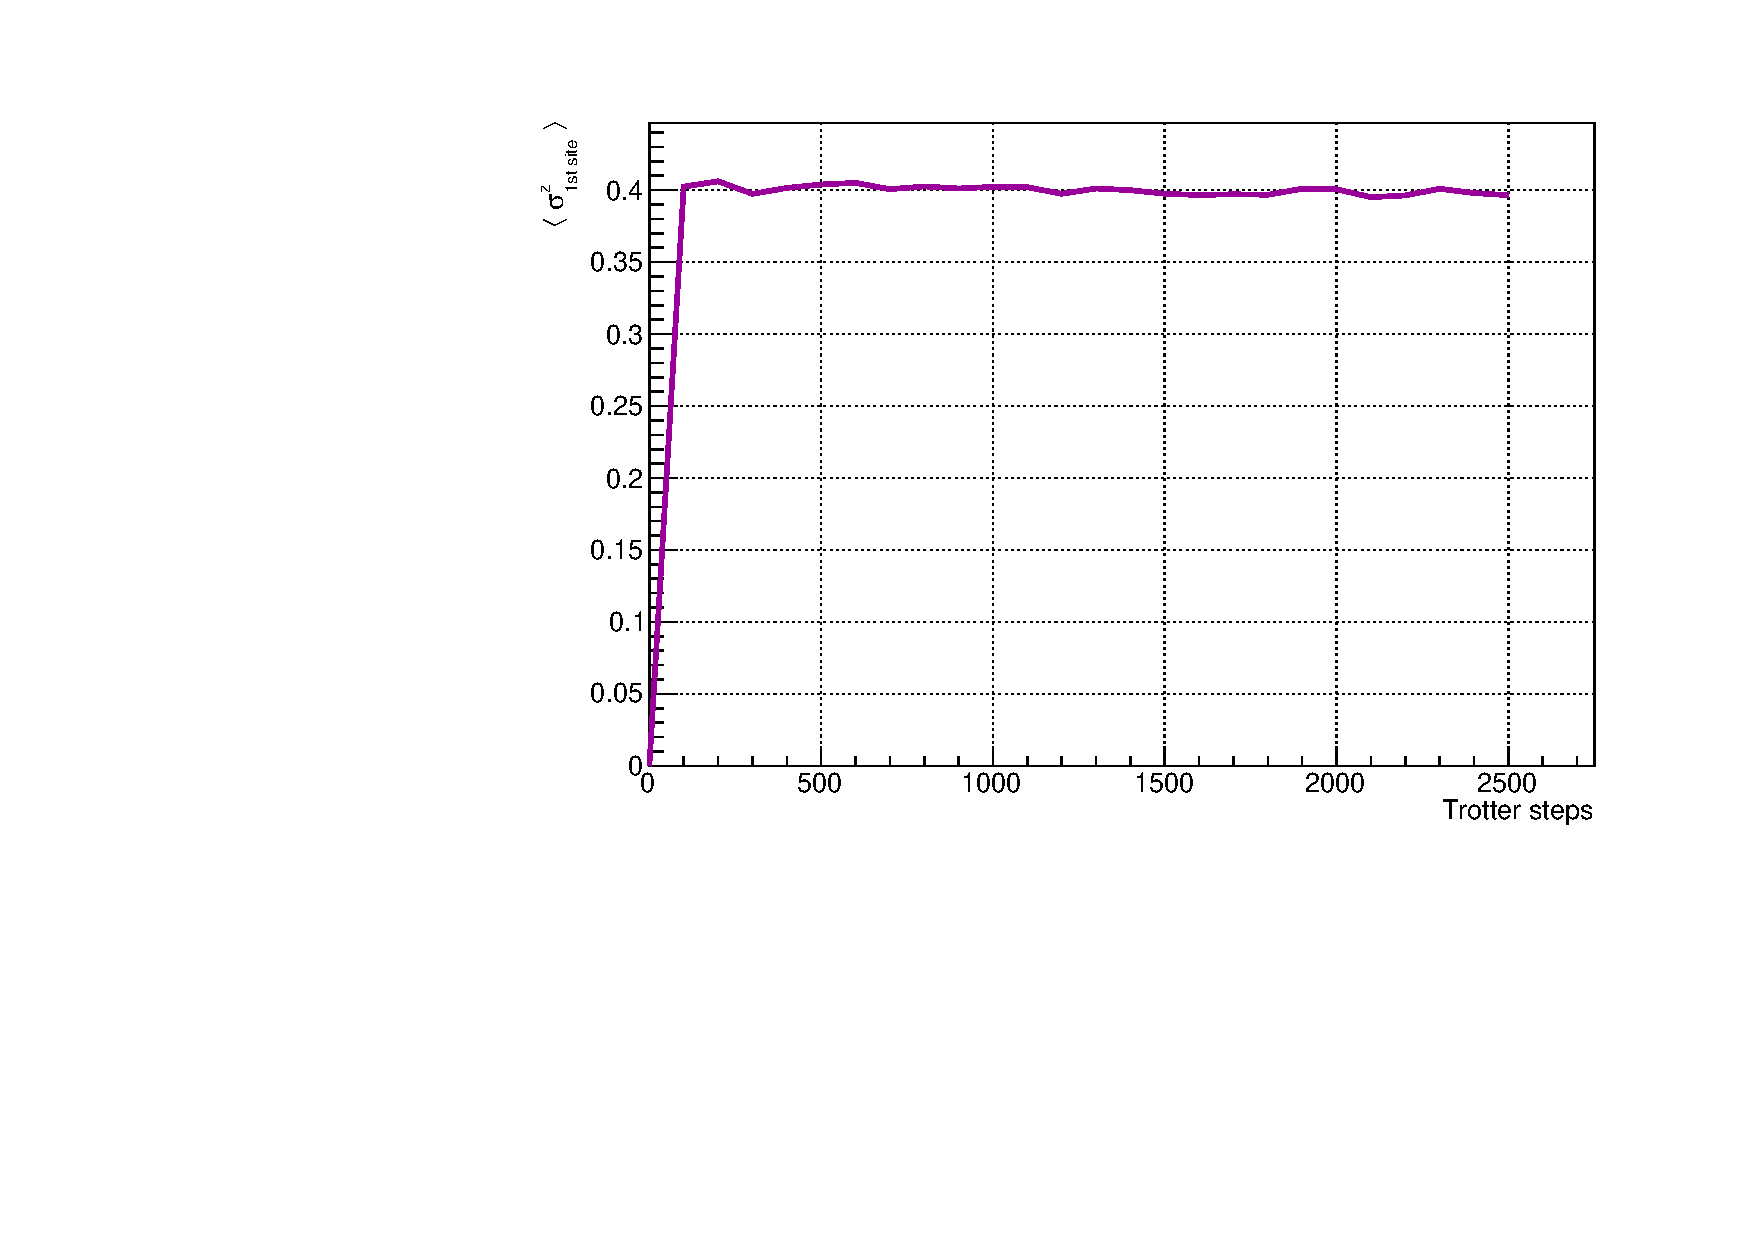
\includegraphics[scale=0.6]{Figures/convergence/ConvergenceLM_L016_m080_Time002500_J1051.pdf}
    \label{fig:16sites_LMvsGamma}
\end{subfigure}\\
\captionsetup{width=1.\linewidth}
\caption{Study of convergence of the MPO method for a 8-sites chain, for bond dimension m = 100 and T = 3000.}
\label{fig:convergence_8_12_16}
\end{figure}

The errors considered for the MPO method are merely the differences between two set of data obtained for two different bond dimension. In particular, the error for an observable $O$ of a 8-sites chain, is given by:
\begin{equation*}
    \epsilon = <O>_{m=100} - <O>_{m=80}.
\end{equation*}

\section{Comparison between QT and MPO results}
As a verification of the plausibility of data obtained from MPO method, we present here a comparison between the data obtained from MPO method and those obtained from QT method.

\begin{figure}
    \centering
        \begin{subfigure}{\columnwidth}
        \centering
        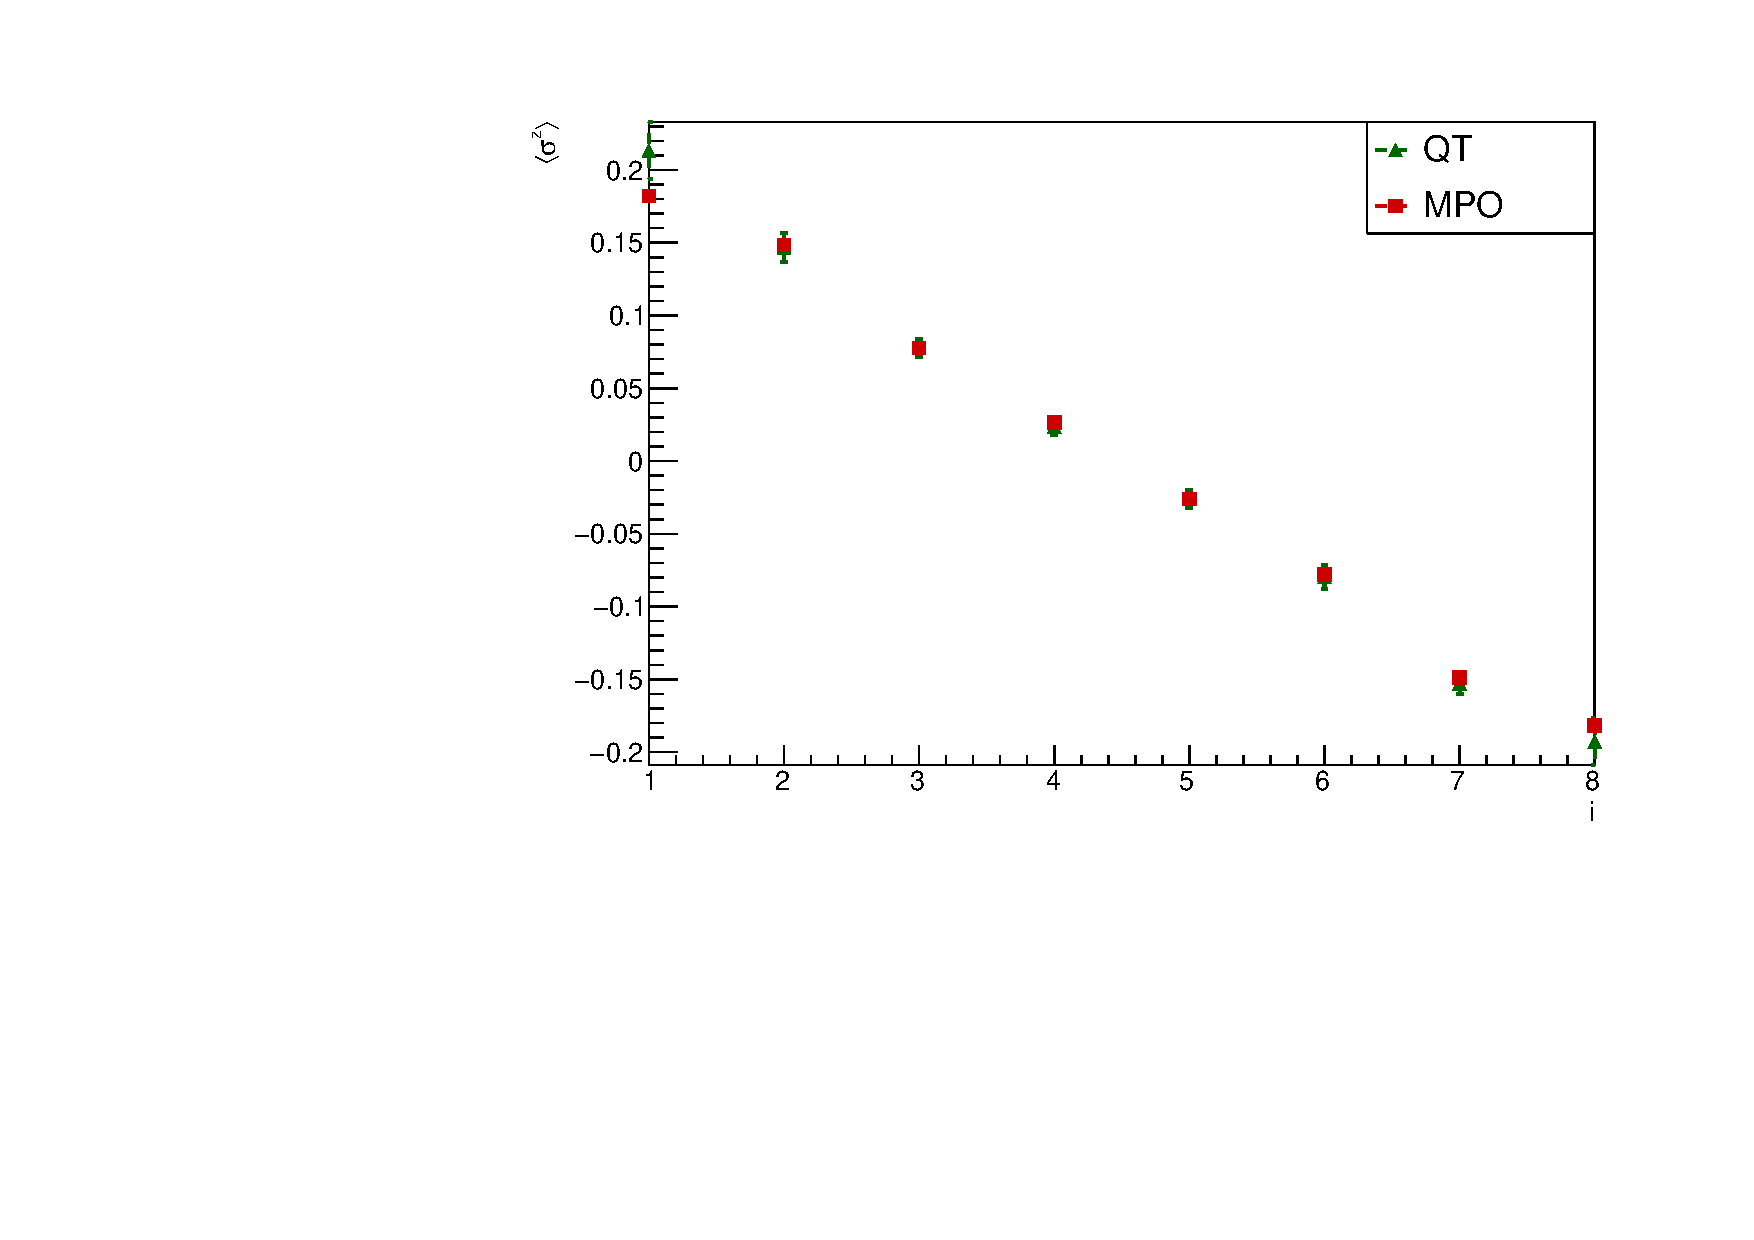
\includegraphics[scale=0.5]{Figures/LMComparison_8sJ10505.pdf}
        \label{fig:LMComparison_8sJ10505}
        \end{subfigure}\\
        \begin{subfigure}{\columnwidth}
        \centering
        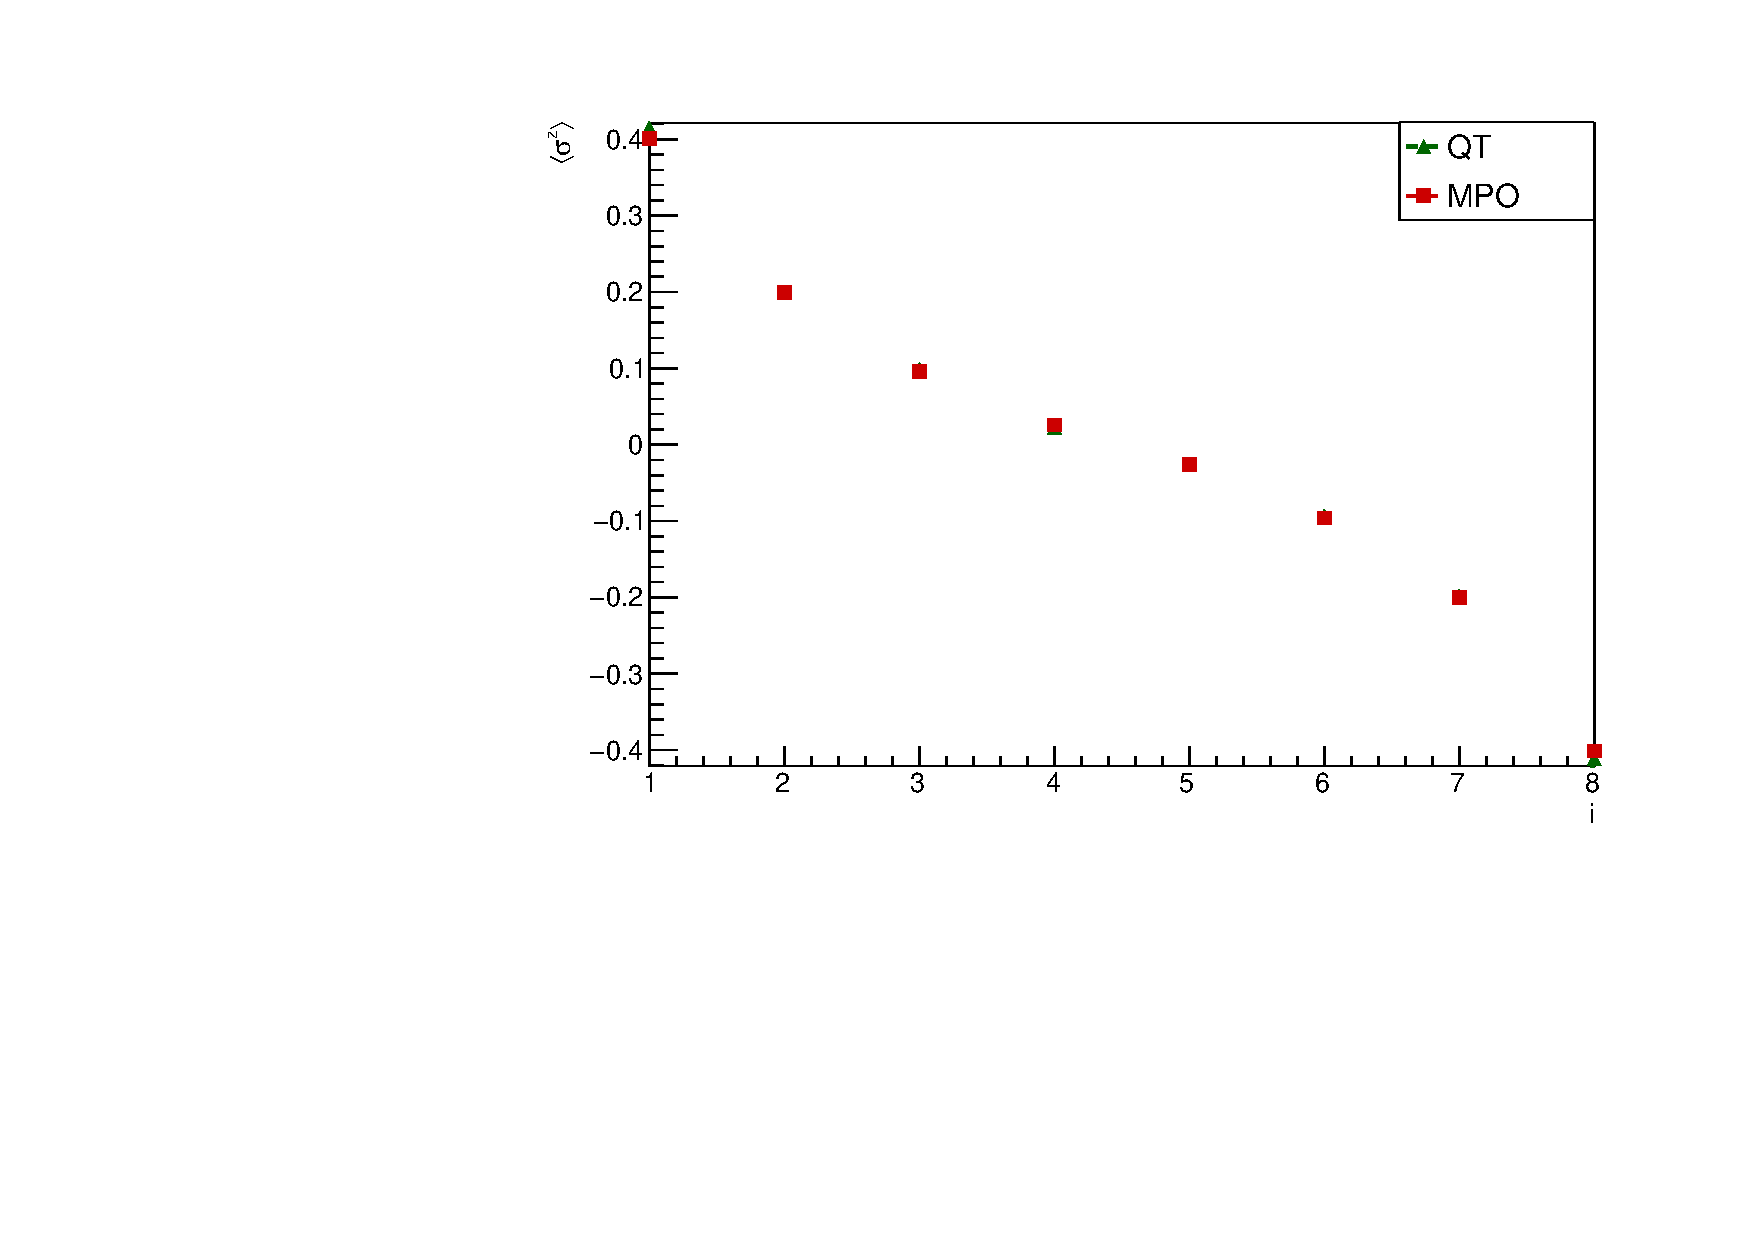
\includegraphics[scale=0.5]{Figures/LMComparison_8sJ1051.pdf}
        \label{fig:LMComparison_8sJ1051}
        \end{subfigure}\\
        \begin{subfigure}{\columnwidth}
        \centering
        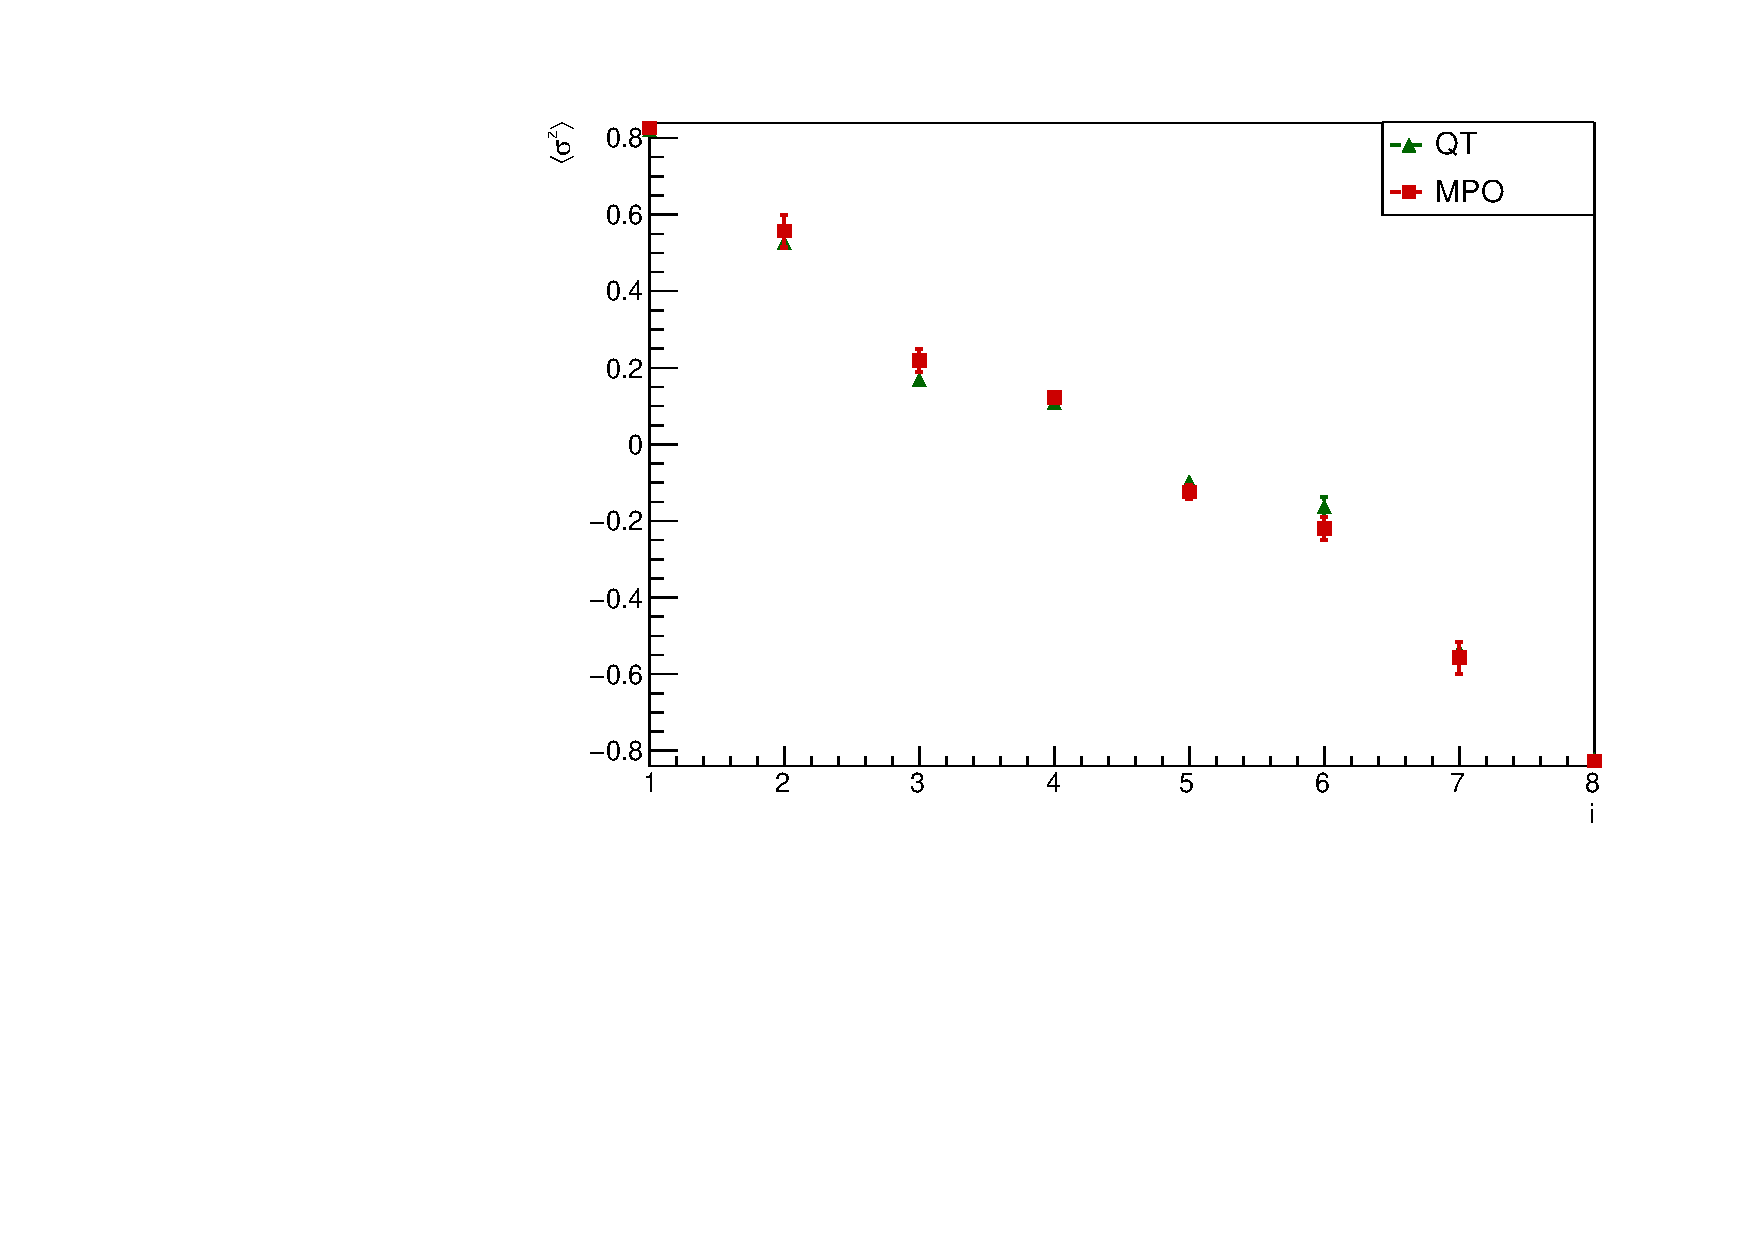
\includegraphics[scale=0.5]{Figures/LMComparison_8sJ10515.pdf}
        \label{fig:LMComparison_8sJ10515}
        \end{subfigure}\\
    \captionsetup{width=1.\linewidth}
    \caption{Magnetization profile for a 8-sites chain for $\gamma = 1$ and $J_z = 0.5$ (upper panel), $J_z = 1$ (middle panel), $J_z = 1.5$ (bottom panel). Data are obtained from MPO method (in red) and QT method (in green).}
    \label{fig:my_label}
\end{figure}


\begin{figure}
    \centering
        \begin{subfigure}{\columnwidth}
        \centering
        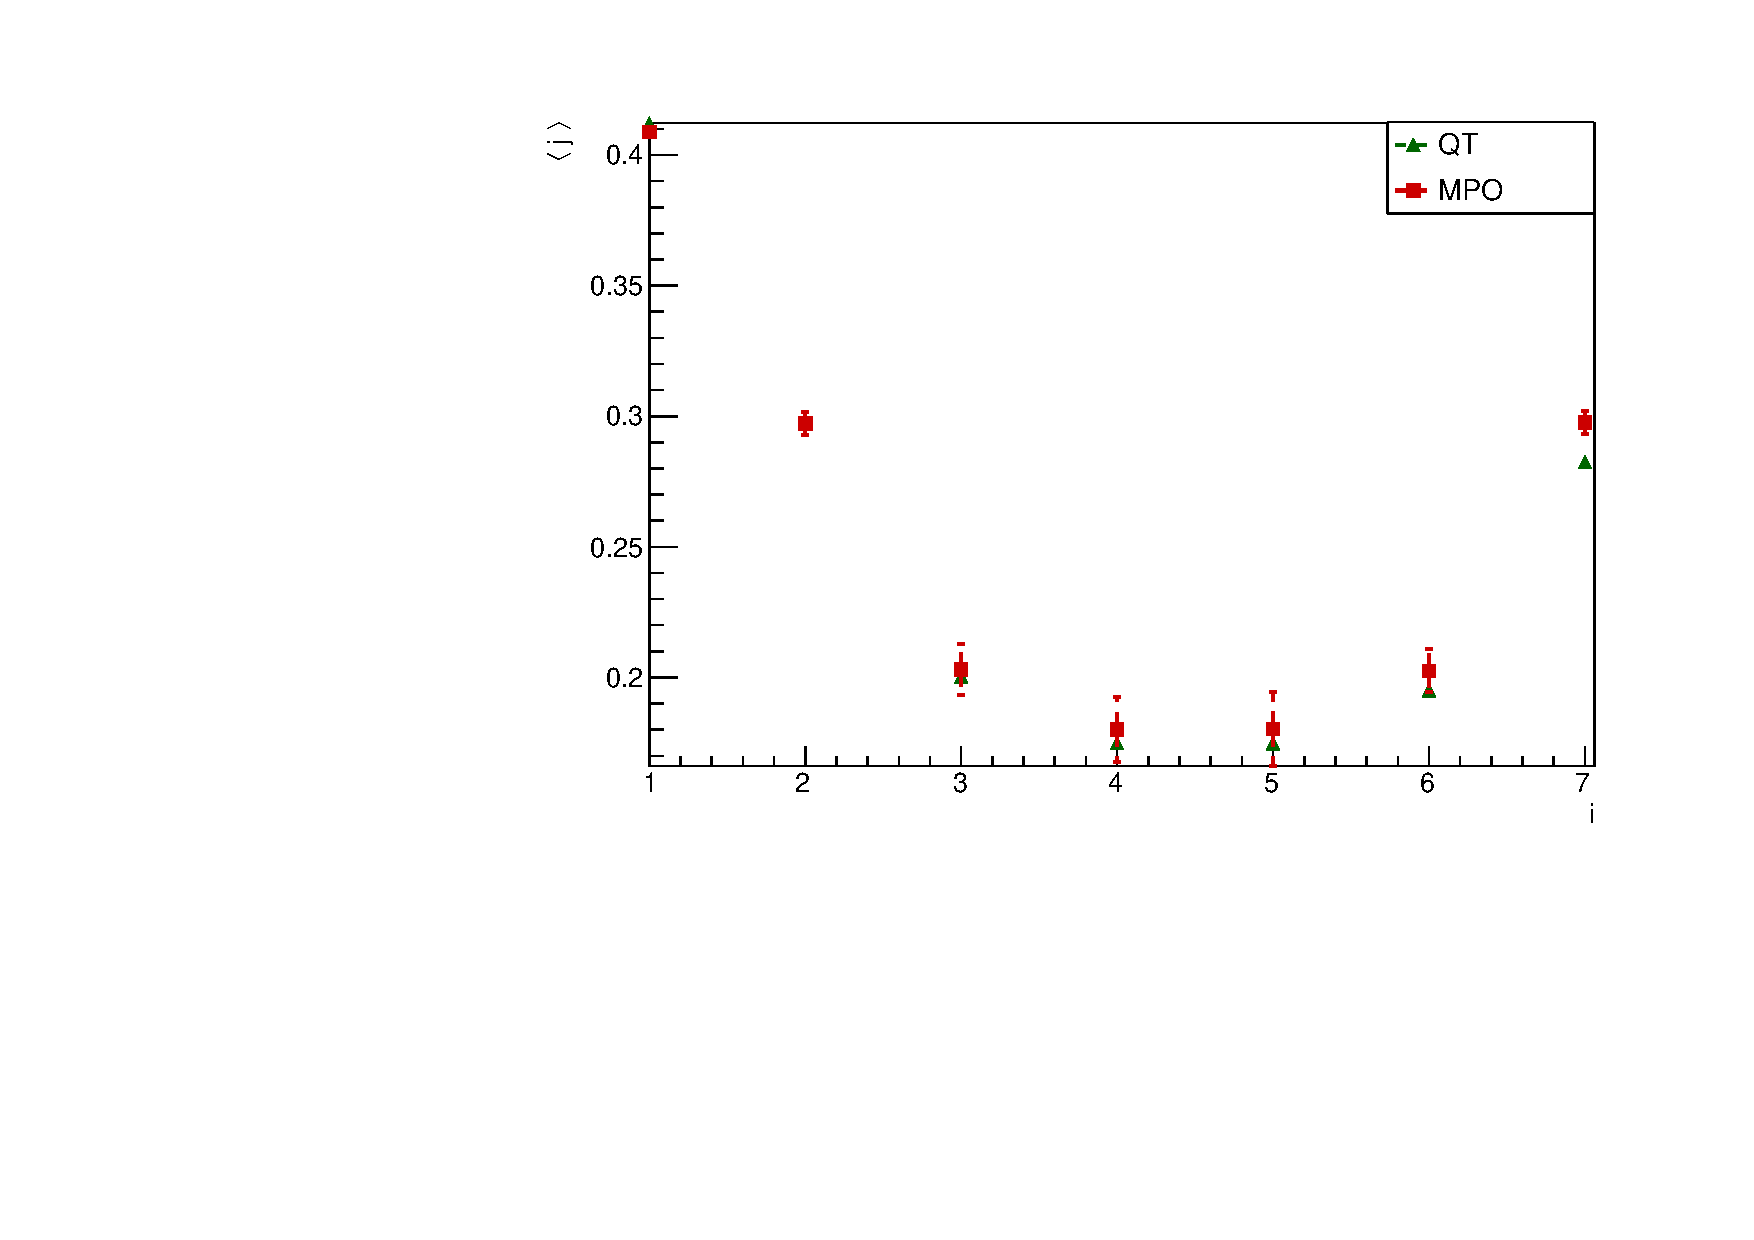
\includegraphics[scale=0.5]{Figures/SpinCurrComparison_8sJ10505.pdf}
        \label{fig:SpinCurrComparison_8sJ10505}
        \end{subfigure}\\
        \begin{subfigure}{\columnwidth}
        \centering
        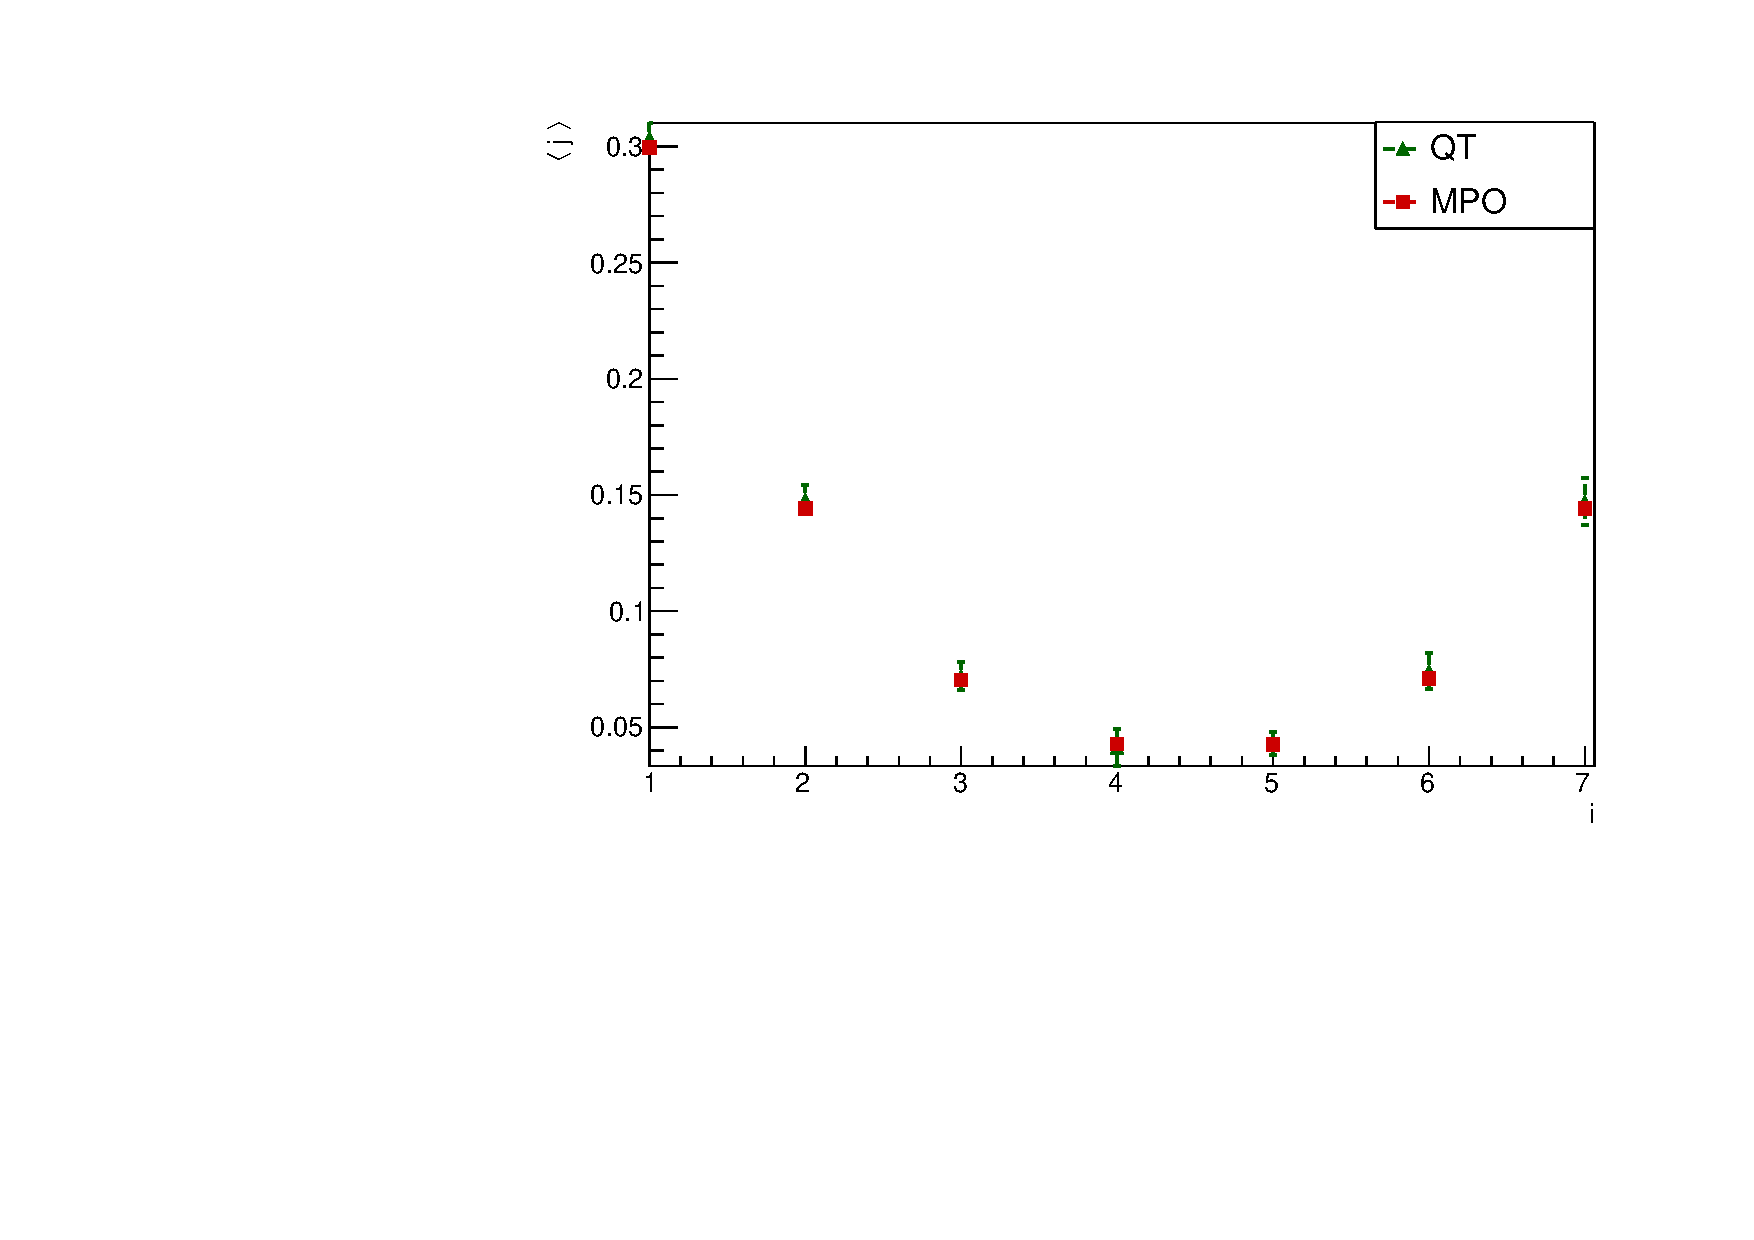
\includegraphics[scale=0.5]{Figures/SpinCurrComparison_8sJ1051.pdf}
        \label{fig:SpinCurrComparison_8sJ1051}
        \end{subfigure}\\
        \begin{subfigure}{\columnwidth}
        \centering
        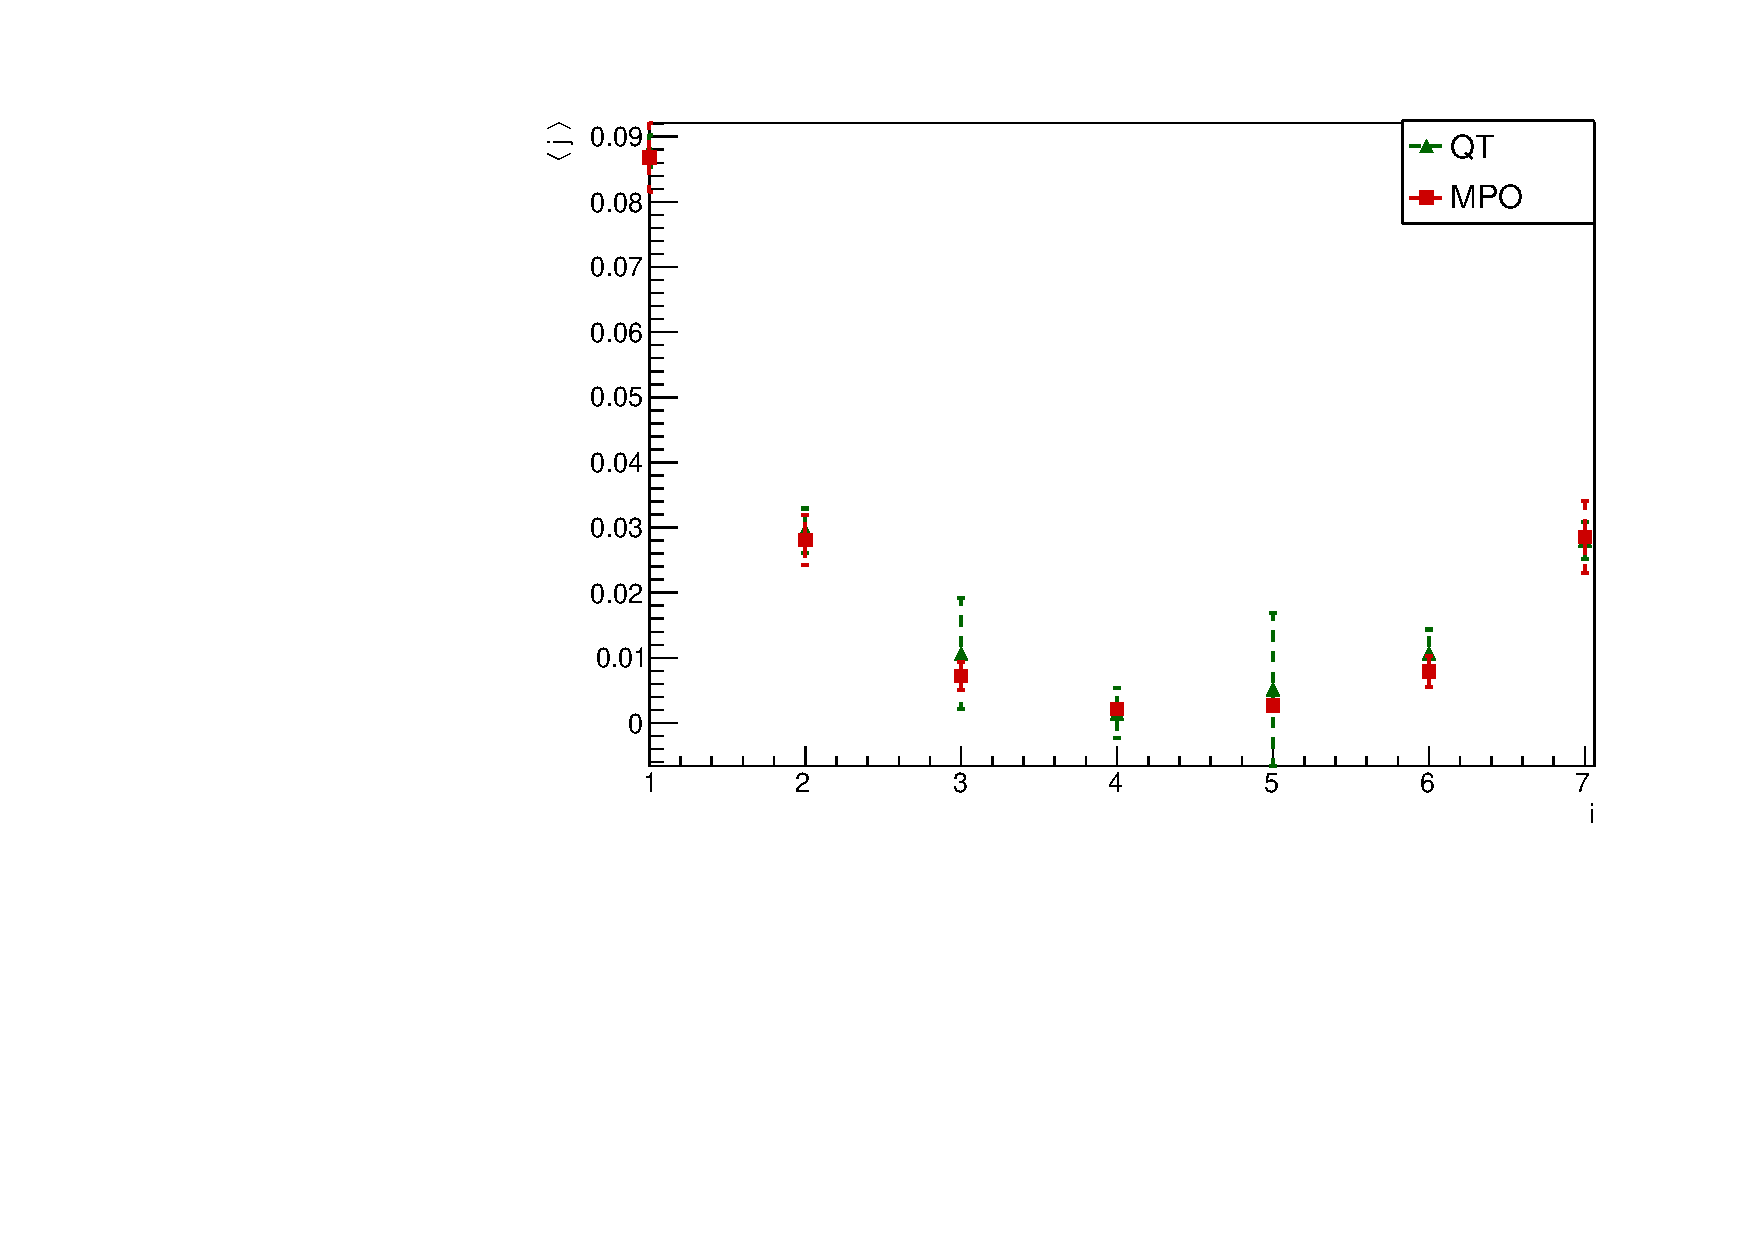
\includegraphics[scale=0.5]{Figures/SpinCurrComparison_8sJ10515.pdf}
        \label{fig:SpinCurrComparison_8sJ10515}
        \end{subfigure}\\
    \captionsetup{width=1.\linewidth}
    \caption{Spin current for a 8-sites chain for $\gamma = 1$ and $J_z = 0.5$ (upper panel), $J_z = 1$ (middle panel), $J_z = 1.5$ (bottom panel). Data are obtained from MPO method (in red) and QT method (in green).}
    \label{fig:my_label}
\end{figure}